%% Based on techreport.tex template as sent by Erik Burger on 2023-11-20
%% 
%% Karlsruhe Institute of Technology
%% Institute for Program Structures and Data Organization
%% Chair for Software Design and Quality (SDQ)
%%
%% Dr.-Ing. Erik Burger
%% burger@kit.edu
%%
%% See https://sdq.kastel.kit.edu/wiki/Dokumentvorlagen
%%
%% Version 1.0, 2023-11-20

%% Available page modes: oneside, twoside
%% Available languages: english, ngerman
%% Available modes: draft, final (see README)
\documentclass[oneside, ngerman]{sdqtechreport}

%% ---------------------------------
%% | Information about the document |
%% ---------------------------------

%% Name of the group and authors
\author{Paul Buda, Martin Scheuermann, Stephan Schneider, \\
Simon Schütz und Nils Seibert}

%% Title (and possibly subtitle) of the thesis
\title{Pflichtenheft}

\subtitle{zur Android-App Neptune}

%% You can put a logo in the ``logos'' directory and include it here
%% instead of the SDQ logo
% \grouplogo{myfile}
%% Alternatively, you can disable the group logo
% \nogrouplogo

\date{01.12.2023}

%% For example texts -- please remove in the final version
\usepackage{blindtext}

%% ====================================
%% ====================================
%% ||                                ||
%% || Beginning of the main document ||
%% ||                                ||
%% ====================================
%% ====================================
\begin{document}

%% Set PDF metadata
\setpdf

%% Set the title
\maketitle

%% ------------------------
%% |   Table of Contents  |
%% ------------------------
\tableofcontents

%% -----------------
%% |   Main part   |
%% -----------------
\cleardoublepage

%% -------------------
%% | Example content |
%% -------------------

\chapter{Einleitung}
\label{chap:Einleitung}

\section{Einführung}
\label{sec:Einleitung:Einführung}
Musik spielt im Leben vieler Menschen eine enorm wichtige Rolle. Insbesondere bei Partys und Zusammenkünften mit Freunden sorgt eine gute Musikauswahl für eine gute Stimmung unter den Anwesenden. Aber auch der umgekehrte Fall ist vielen sicherlich gut bekannt – gefällt die abgespielte Musik den Anwesenden nicht, so kann dies die Stimmung erheblich trüben.

Nahezu alle der heute gängigen Musikstreaming-Anbieter versuchen bereits mit proprietären Lösungen, dem entgegenzuwirken. In der Praxis jedoch sind die eigens von den Anbietern angebotenen Lösungen häufig nicht praktikabel. Die Ursachen hierfür sind divers, so setzen die von den Anbietern selbst entwickelten Tools häufig voraus, dass alle Teilnehmer über ein bestehendes Abonnement beim entsprechenden Anbieter verfügen. 

Das Ziel des Projekts ''Neptune'' ist es, eine praktikable Lösung für die eingangs beschriebene Problematik anzugeben. Hierzu soll im Rahmen des Moduls ''Praxis der Softwareentwicklung'' eine Android-App entwickelt werden, mithilfe derer über die bei einer Party oder einem vergleichbaren Event abgespielte Musik entschieden werden kann.

Hierzu sollen die Anwesenden in verschiedenen verfügbaren Abstimmungs-Modi Musikvorschläge einbringen und über diese abstimmen können. Die Musik soll dann über das Endgerät einer weiteren anwesenden Person, des sogenannten ''Hosts'', abgespielt werden. 
Mittels der Einbindung eines gängigen Musikstreaming-Service soll die App in die Lage versetzt werden, einen breiten Musikkatalog bereitzustellen.


\section{Anwendungsbereich}
\label{sec:Einleitung:Anwendungsbereich}

Das Ziel von Neptune ist es, die Musikauswahl bei privaten Veranstaltungen, wie zum Beispiel studentische WG- und Wohnheimpartys, einfacher und gerechter zu gestalten.
Die Android-App Neptune bietet Gruppen die Möglichkeit jeden an der Musikauswahl zu beteiligen und über die Abspielreihenfolge demokratisch abzustimmen. Durch die Integration mit einem Audio-Streaming-Dienst wie Spotify kann Neptune automatisch die am besten bewerteten Songs abspielen. Damit ist es möglich Songwünsche von Gästen zu erfüllen, ohne einen aktiven ''DJ''  der die Wünsche entgegen nimmt und sie manuell in die Warteschlange hinzufügt.

Bei der Erstellung einer Listening-Session kann der Gastgeber die verfügbaren Lieder nach Belieben auf verschiedene Genres oder eine Playlist beschränken. Nach Auswahl des Modus kann der Gastgeber die Gäste einladen, sich an der Musikauswahl zu beteiligen, indem er einen sechsstelligen Zahlencode oder einen Link weitergibt. Die Gäste können dann in der App Lieder in die Vorschlagsliste hinzufügen und mit dem Verteilen von Upvotes Lieder in der Liste nach oben voten und sie somit schneller zum Abspielen bringen. Der Host hat durch eine Kontrollansicht einen Überblick über die Queue, sowie die Vorschlagsliste in Neptune. Er kann in dieser Ansicht Songs in die Queue hinzufügen und entfernen, sowie Lieder aus der Vorschlagsliste entfernen, dadurch hat der Host weiterhin die volle Kontrolle über die Musikauswahl. Zusätzlich kann er durch die Einstellung
eines Cooldowns verhindern das diesselben Songs mehrmals mit geringen Abstand gespielt werden.

Eine vollständige Beschreibung der Anwendungsfälle sind  den \hyperlink{Anwendungsfaelle}{Use Case Diagrammen} zu entnehmen   


\section{Zielgruppe}
\label{sec:Einleitung:Zielgruppe}

Die primäre Zielgruppe von Neptune besteht aus Veranstaltern und Besuchern von Privatpartys, die zwischen 5-50 Besucher haben. Das Alter der Zielgruppe liegt dabei bei 18-35 Jahren, in dieser Altersgruppe ist von Vertrautheit bei der Bedingung von Smartphoneapps auszugehen. Darüber hinaus haben eine Mehrheit in dieser Altersgruppe einen Zugang zu Spotify, sowie ein aktuelles Smartphone. Dadurch sind die Zugangsbarrieren für die Benutzung von Neptune sehr niedrig.

Auch für Menschen außerhalb dieser primären Zielgruppe kann Neptune durch sein flexibles und einfaches Design interessant sein. Zum Beispiel ist mit der App auch möglich über die perfekte Entspannungsmusik beim Yoga abzustimmen oder das beliebteste Weihnachtslied in der Großfamilie zu ermitteln. 
Im Rahmen dieses PSE-Projekt wird die Zielgruppe auf Androidbenutzer eingeschränkt.

\chapter{Zielbestimmungen}
\label{chap:Zielbestimmungen}

\section{Musskriterien}
\label{sec:Zielbestimmungen:Musskriterien}
\begin{itemize}
    \item Mithilfe des Systems sollen User gemeinsam auf Veranstaltungen live über die während der Veranstaltung abgespielte Musik abstimmen bzw. entscheiden können.
    \item Hauptbestandteil des Systems ist ein Abstimmungssystem, welches Participants das Vorschlagen von Tracks ermöglicht. Dazu stellt das System verschiedene Modi zu Auswahl.
    \begin{itemize}
        \item Participants können bezüglich bereits vorgeschlagener Tracks ein Upvote abgeben. Je nach gewähltem Abstimmungsmodus hat die jeweilige Anzahl der Upvotes eines Tracks Einfluss darauf, ob und wann er abgespielt wird.
    \end{itemize}
    \item Das System ist in der Lage, Usern einen durchsuchbaren Musikkatalog zur Verfügung zu stellen. Diese werden über entsprechende, auf dem Markt verfügbare Schnittstellen externer Anbieter bereitgestellt. Konkret wird dies im System durch die Einbindung mindestens einer externen API-Schnittstelle eines Musikstreaming-Anbieters realisiert.
    \begin{itemize}
        \item Das im Rahmen des Moduls ''Praxis der Softwareentwicklung'' zu entwickelnde System beschränkt sich hierbei auf einen konkreten Musikstreaming-Anbieter, namentlich auf das Angebot des schwedischen Unternehmens Spotify. Hierbei soll die Möglichkeit zur einfachen komplexen Ausweitung des Systems auf weitere Musikstreaming-Anbieter gegeben sein.
        \begin{itemize}
            \item Aufgrund von Einschränkungen seitens Spotify bezüglich der Entwicklerarbeit mit der von Spotify bereitgestellten API ist die vorgesehene Anzahl zulässiger User innerhalb einer gemeinsamen Session zunächst auf 25 User beschränkt.
            \item Aufgrund der Eigenschaften der Spotify-API ergibt sich darüber hinaus, dass für User ohne Spotify-Account sowie User ohne einen Spotify-Account mit einem Premium-Abonnement vorgesehen ist, dass diese nicht selbst neue Songs in der App vorschlagen können. Jedoch können diese User über von anderen Usern vorgeschlagene Songs abstimmen.
        \end{itemize}

        \end{itemize}
    \item Für eine Veranstaltung kann eine sogenannte Session durch den Host erstellt werden. Participants können dieser mithilfe eines sechsstelligen Beitrittscodes beitreten. Alle Entscheidungen über abzuspielende Musik finden innerhalb der Session statt.
    \item Das System verwendet zur Entscheidung über abzuspielende Songs ein nach diversen Kriterien konfigurierbares Abstimmungssystem.
    \begin{itemize}
        \item Zum einen sind verschiedene Abstimmungsmodi vorgesehen:
        \begin{itemize}
            \item General Mode
            \begin{itemize}
                \item Full Participants sowie der Host können im bereitgestellten Musikkatalog einen beliebigen Track auswählen und diesen vorschlagen
                \item Participants haben die Möglichkeit, einem Track ein Upvote zu geben. Hat ein Participant bereits selbst ein Upvote an einen Track vergeben, so ist es ihm möglich, dieses wieder zu entfernen.
                \item Der Host kann einen Track, welcher ein Upvote erhalten hat, zur Queue hinzufügen. Außerdem hat er die Möglichkeit, Tracks zu sperren.
            \end{itemize}
            \item Artist Mode
            \begin{itemize}
                \item Die Grundfunktionalität ist gleich der des General Modes. Hierbei legt der Host jedoch zuvor eine Liste an erlaubten Artists fest. Während der gesamten Session kann ein Track ausschließlich dann in der Suche gefunden, vorgeschlagen werden, Upvotes erhalten und abgespielt werden, wenn er mindestens einem der erlaubten Artists zugeordnet werden kann.
            \end{itemize}
            \item Genre Mode
            \begin{itemize}
                \item Die Grundfunktionalität ist gleich der des General Modes. Hierbei legt der Host jedoch zuvor eine Liste an erlaubten Genres fest. Während der gesamten Session kann ein Track ausschließlich dann in der Suche gefunden, vorgeschlagen werden, Upvotes erhalten und abgespielt werden, wenn er mindestens einem der erlaubten Genres zugeordnet werden kann.
            \end{itemize}
            \item Playlist Mode
            \begin{itemize}
                \item Die Grundfunktionalität ist gleich der des General Modes. Hierbei hinterlegt der Host jedoch zuvor eine Playlist, welche von dem für die Session genutzten Musikstreaming-Anbieter stammt. Während der gesamten Session kann ein Track ausschließlich dann in der Suche gefunden, vorgeschlagen werden, Upvotes erhalten und abgespielt werden, wenn er in der hinterlegten Playlist enthalten ist.
            \end{itemize}
        \end{itemize}

    \end{itemize}
    \item Die User können genau eine der untenstehend aufgeführten Rollen bekleiden. Je nach der individuellen Ausgestaltung der Abstimmungsmodi ist die Rolle eines Users entscheidend in Hinblick auf die Entscheidungsfindung zur abzuspielenden Musik.
    \begin{itemize}
        \item Host: Der Host ist der Ersteller einer Session. Auf der einen Seite verwaltet er sie und kann sie auflösen, auf der anderen Seite wird die abzuspielende Musik über sein Endgerät abgespielt.
        \item Participant: Alle Teilnehmer einer Session, welche nicht der Host sind, bekleiden automatisch die Rolle Participant. Participants können basierend auf den gewählten Abstimmungsparametern neue Songs vorschlagen und/oder über vorgeschlagene Songs abstimmen. 
    \end{itemize}
    \item Die abzuspielende Musik wird über externe Anbieter abgespielt. Hierbei wird analog zur Einbindung von Musikstreaming-Anbietern bereitgestellter externer Schnittstellen vorgegangen.
    \item  Den Usern stehen für die Bedienung und das User-Interface der App folgende Sprachen zur Verfügung, zwischen welchen sie frei wechseln können:
    \begin{itemize}
        \item Englisch: Durch die weite Verbreitung der englischen Sprache sorgt ihre Unterstützung innerhalb der App dafür, dass die erreichbare Zielgruppe stark wächst, ohne direkt nativ eine Vielzahl von Sprachen unterstützen zu müssen.
        \item Deutsch: \textit{(--> muss hier eine Begruendung hin?)}
    \end{itemize}
\end{itemize}
\section{Wunschkriterien}
\label{sec:Zielbestimmungen:Wunschkriterien}
\begin{itemize}
    \item Jeder User soll in einer Statistikansicht Informationen über die Session einsehen können. Diese Ansicht wird automatisch beim Verlassen der Session angezeigt. Während der Session kann sie durch ein Button geöffnet werden. Die Statistik soll als Bild exportierbar und teilbar sein. 
    Folgende Datenpunkte sollen dabei angezeigt werden. 
    \begin{itemize}
        \item Song mit meisten Votes der Session
        \item Genre mit den meisten Votes der Session
        \item Artist mit den meisten Votes der Session
        \item Anzahl abgespielte Songs in der Session
        \item Dauer der Session
        \item Anzahl Teilnehmer in der Session 
        \item Verteilte Herzen in Session
    \end{itemize}
  
    \item Im Falle dessen, dass die Teilnehmer keine neue Musik vorschlagen und die Warteschlange hierdurch leer ist, soll die App mittels einer Autoplay-Funktion dennoch kontinuierlich Musik abspielen.
    \item QR-Code (6stelliger Code in Musskrit)

\end{itemize}

\section{Abgrenzungskriterien}
\label{sec:Zielbestimmungen:Abgrenzungskriterien}
\begin{itemize}
    \item Musik soll nicht innerhalb der App selbst abgespielt werden.
    \item Im Rahmen des Projekts soll keine öffentlich zugängliche API und insgesamt keine Schnittstelle für weitere externe Anwendungen bereitgestellt werden
    \item Die App soll, abgesehen von einer Internetverbindung, keine weiteren alternativen Netzwerktechnologien wie Bluetooth o.ä. nutzen.
    \item Die App unterstützt nur den Portrait-Modus, nicht den Landscape-Modus.

\end{itemize}




\chapter{Benutzeroberfläche}
\label{chap:Benutzeroberfläche}

\section{Allgemeines}
\label{sec:Benutzeroberfläche:Allgemeines}
Die Benutzeroberfläche wird so gestaltet, dass diese einfach, intuitiv und ohne Vorkenntnisse von Nutzern der Zielgruppe verwendet werden kann. Näheres findet sich unter Benutzerfreundlichkeit im Kapitel Qualitätszielbestimmungen (\ref{Qualitätszielbestimmungen_Benutzerfreundlichkeit}).

Beim Starten der App, wenn die App vollständig beendet ist/war, öffnet sich eine von drei Views:
\begin{itemize}
    \item Die userVoteView (REF) öffnet sich, wenn man derzeit Participant einer aktiven Session ist.
    \item Die hostControlView (REF) öffnet sich, wenn man derzeit Host einer aktiven Session ist.
    \item Die startView (REF) öffnet sich, wenn man derzeit nicht Participant oder Host einer aktiven Session ist.
\end{itemize}
Falls die App nicht vollständig beendet wurde und die Zustandsdaten des Android-Betriebssystems noch vorhanden sind, so öffnet sich die App in der Ansicht, in der man sie verlassen hat.



\newpage

\section{Grafikentwürfe und funktionale Anforderungen}
\label{sec:Benutzeroberfläche:Grafiken}
% do not show subsections in contents
\addtocontents{toc}{\protect\setcounter{tocdepth}{1}}

Die folgenden Grafikentwürfe sind nur erste Entwürfe. Sie sollen einen ersten Eindruck vom Aussehen der App vermitteln und vor allem die ''Topologie'' der App darstellen: Das heißt, wo sich welche Buttons befinden und was diese bewirken. Wir möchten ausdrücklich klarstellen, dass wir die hier gezeigten Designs hinsichtlich Formen, Farben und Anordnung noch verändern wollen und werden. Die Designs sind nicht als final zu verstehen.

In den folgenden Unterkapiteln finden sich alle Views der App. Der Unterkapitelaufbau ist folgendermaßen: Jede View enthält einen Grafikentwurf, eine grobe textuelle Erläuterung und die detaillierte Definition aller wichtigen Benutzeroberflächen-Elemente. Das Klicken selbst und das Verhalten nach dem Klicken auf ein klickbares solches Element ist stets als funktionale Anforderung zu verstehen.


\subsection{Startseite (startView)}
\label{sec:Benutzeroberfläche:startView}

\begin{minipage}{0.5\textwidth}
    \hypertarget{startView}{}
    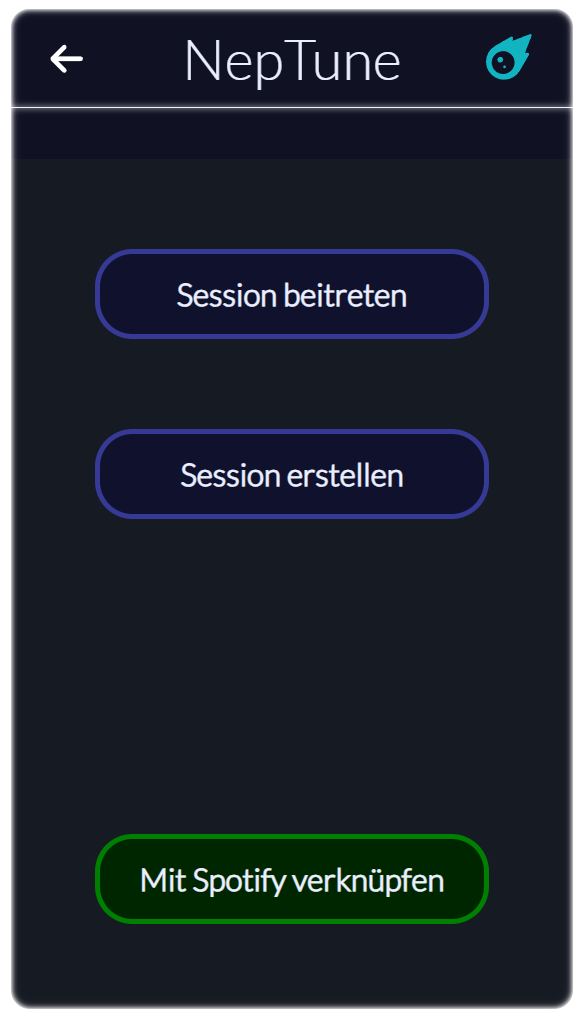
\includegraphics[width=0.9\textwidth]{LATEX/Pflichtenheft/GraphicDesigns/startPage.png}
    \captionof{figure}{startView}
\end{minipage} 
\hfill
\begin{minipage}{0.5\textwidth}
    Beim Öffnen der App soll der User mit möglichst wenigen Optionen konfrontiert werden. Ihm Stehen nur das Verlassen der App, der Beitritt einer Session, das Erstellen einer Session (falls bereits mit Spotify-Premium-Account verknüpft) und das Verwalten der Spotify-Verknüpfung zur Auswahl. 
\end{minipage}
\vspace{\baselineskip}

\newpage
\textbf{Session beitreten:}
\begin{itemize}
    \item Solange der User sich nicht mit einem Spotify-Account verknüpft hat, wird darunter ein Hinweis angezeigt, dass User ohne verknüpften Account nur über von anderen Usern vorgeschlagene Tracks abstimmen können und zum Vorschlagen ein verknüpfter Spotify-Account benötigt wird.
    \item Durch Klicken des Buttons ''Session beitreten" gelangt der Nutzer auf die \hyperlink{userJoinGroupPage}{userJoinGroupPage}. Dabei wird er zum Full Participant, wenn er mit einem Spotify-Account verknüpft ist. Anderfalls wird er zu einem Restricted Partcipant.
\end{itemize}

\textbf{Session erstellen:}
\begin{itemize}
    \item Der Button ''Session erstellen'' ist so lange deaktiviert und ''verblasst'', bis sich der Nutzer über den Button ''Mit Spotify verknüpfen'' erfolgreich mit einem Spotify-Premium-Account verknüpft hat. Danach wird er funktionsfähig.
    \item Solange der Button ''Session erstellen'' deaktiviert ist, wird darunter ein Hinweis angezeigt, dass das Erstellen einer Session nu mit einem verknüpften Spotify-Premium-Account möglich ist.
    \item Durch Klicken des funktionsfähigen Buttons ''Session erstellen'' gelangt der Nutzer auf die \hyperlink{hostModusSelectPage}{hostModusSelectPage}.
\end{itemize}

\textbf{Mit Spotify verknüpfen:}
\begin{itemize}
    \item Durch Klicken des Buttons ''Mit Spotify verknüpfen'' verknüpft sich die App wenn möglich automatisch und im Hintergrund mit dem lokal angemeldeten Spotify-Account. Ist dies nicht möglich öffnet sich die von Spotify zur Verfügung gestellte Anmeldemaske, um per Login seinen Account zu verknüpfen.
    \item Nach dem erfolgreichen Verknüpfen mit Spotify, ändert sich die Beschriftung des Buttons von ''Mit Spotify verknüpfen'' zu ''Von Spotify trennen''.
    \item Durch Klicken des Buttons ''Von Spotify trennen'' wird das Spotify Konto des Nutzers wieder von NepTune getrennt.
    \item Nach dem erfolgreichen Trennen von Spotify, ändert sich die Beschriftung des Buttons von ''Von Spotify trennen'' zu ''Mit Spotify verknüpfen''.
\end{itemize}

\textbf{Zurück-Button:}
\begin{itemize}
    \item Beim Klicken des Zurück-Buttons erscheint ein Pop-Up Fenster mit der Frage ''NepTune wirklich schließen?''. In diesem Pop-Up kann sich der Nutzer nun zwischen ''Ja'' und ''Nein'' entscheiden.
    \begin{itemize}
        \item Durch Auswählen von ''Ja'' verlässt der User die App und die App wird beendet.
        \item Durch Auswählen von ''Nein'' bleibt der User in der \hyperlink{startView}{startView}.
    \end{itemize}
\end{itemize}


\newpage

\subsection{Sessionbeitritt (joinSessionView)}
\label{sec:Benutzeroberfläche:joinSessionView}


\begin{minipage}{0.5\textwidth}
    \hypertarget{joinSessionView}{}
    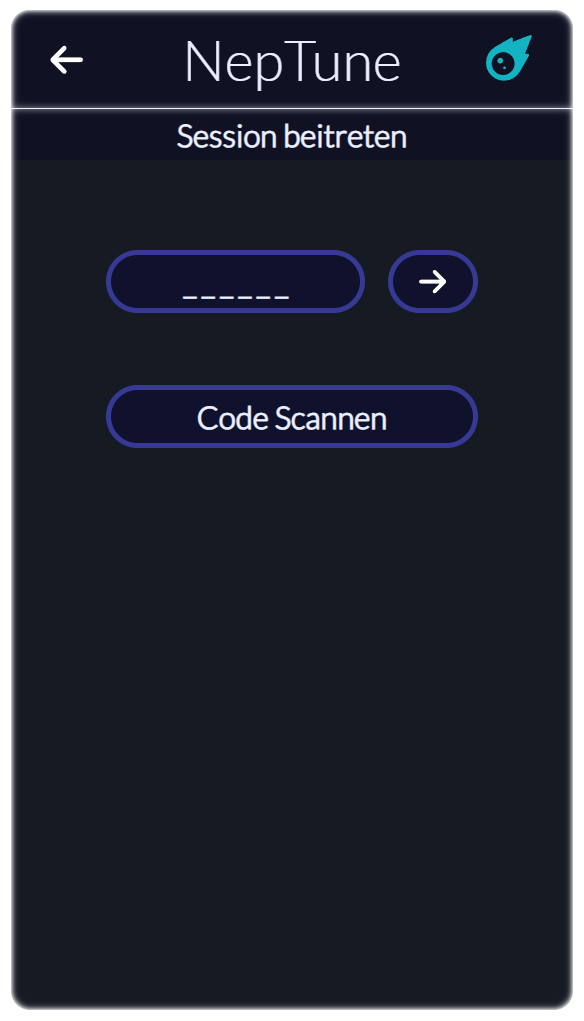
\includegraphics[width=0.9\textwidth]{LATEX/Pflichtenheft/GraphicDesigns/userJoinGroupPage.png}
    \captionof{figure}{joinSessionView}
\end{minipage} 
\hfill
\begin{minipage}{0.5\textwidth}
    Zum Beitritt einer Session als Full Participant (mit verknüpftem Spotify-Account) oder Restricted Participant (mit verknüpften Spotify-Account) muss der User einen gültigen Session-Code eingeben oder einen gültigen QR-Code einscannen. Die Möglichkeit dazu bietet ihm diese View.
\end{minipage}
\vspace{\baselineskip}

\textbf{Code-Eingabefeld:}
\begin{itemize}
    \item Eingabefeld zur Eingabe des sechsstelligen Codes, der die Session eindeutig identifiziert.
\end{itemize}

\textbf{Code bestätigen:}
\begin{itemize}
    \item Existiert eine Session zum eingegebenen sechsstelligen Code, führt Klicken des Bestätigungsbuttons auf die \hyperlink{userVotePage}{userVotePage} der Session.
    \item Existiert keine Session zur Eingabe, erscheint ein entsprechender Hinweis unter dem Code-Eingabefeld und der Inhalt des Code-Eingabefeldes wird gelöscht.
\end{itemize}

\textbf{Code scannen:}
\begin{itemize}
    \item Durch Klicken des Buttons ''Code scannen'' öffnet sich ein QR-Code-Reader. Nach dem erfolgreichen Scannen eines gültigen QR-Codes gelangt man ebenfalls auf die \hyperlink{userVotePage}{userVotePage} der Session.
    \item Der sich nach dem Klicken öffnende QR-Code-Reader besitzt einen Button zum Schließen.
    \item Der sich nach dem Klicken öffnende QR-Code-Reader zeigt eine Meldung mit entsprechendem Hinweis an, falls ein erfolgreich gelesener QR-Code keinen gültigen Session-Code darstellt.
\end{itemize}

\textbf{Zurück-Button:}
\begin{itemize}
    \item Durch Klicken des Zurück-Buttons gelangt man auf die \hyperlink{startView}{startView}.
\end{itemize}

\newpage

\subsection{Abstimmungsansicht einer Session (sessionVoteView)}
\label{sec:Benutzeroberfläche:joinSessionView}


\begin{minipage}{0.5\textwidth}
    \hypertarget{sessionVoteView}{}
    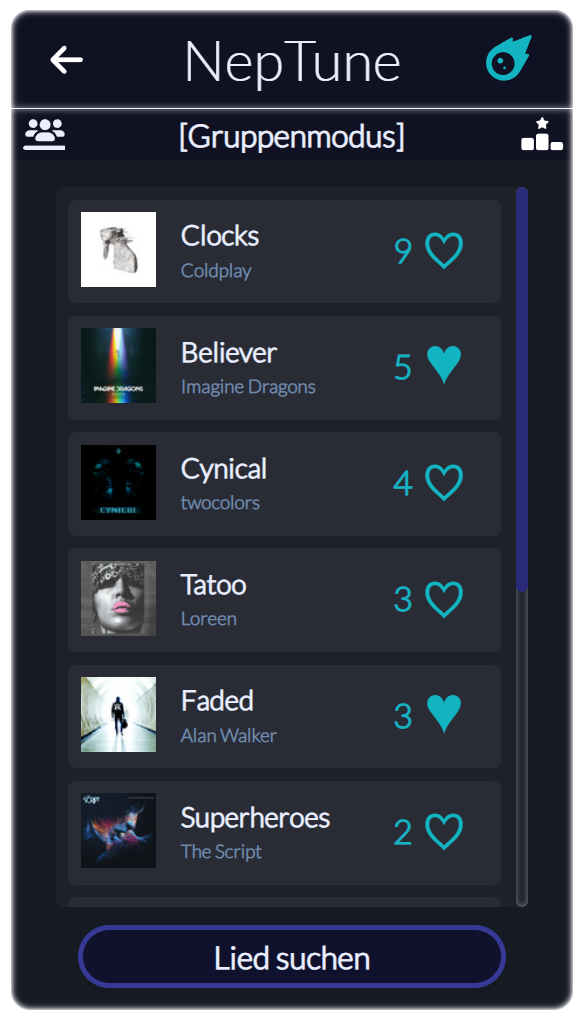
\includegraphics[width=0.9\textwidth]{LATEX/Pflichtenheft/GraphicDesigns/userVotePage.png}
    \captionof{figure}{sessionVoteView}
\end{minipage} 
\hfill
\begin{minipage}{0.5\textwidth}
    XXX
\end{minipage}

\textbf{Session-Info:}
\begin{itemize}
    \item Durch Klicken auf den Button Session-Info (der mit dem Gruppen-Icon) gelangt man in die sessionInfoView (REF).
\end{itemize}

\textbf{Statistiken:}
\begin{itemize}
    \item Durch Klicken auf den Button Session-Info (der mit dem Balken-Icon) gelangt man in die sessionStatsView (REF).
\end{itemize}

\textbf{Track-Anzeige:}
\begin{itemize}
    \item Grundsätzlich nicht klickbare (außer dem Track-Upvote-Button) Liste von Tracks mit mindestens einem Upvote. \item Jeder Track wird mit Cover, Titel, Interpret und der Anzahl der Upvotes angezeigt, sowie der Information, ob der User den Track geupvotet hat.
    \item Ausnahme: Im Playlist Mode werden alle Tracks der Playlist angezeigt, auch solche ohne Upvote.
\end{itemize}

\textbf{Track-Upvote:}
\begin{itemize}
    \item Durch Klicken des Track-Upvote-Buttons eines Tracks (der mit dem Herz) erhöht sich der Counter der Upvotes des Tracks und das Herz wird ausgefüllt.
    \item Durch erneutes Klicken des bereits geklickten Track-Upvote-Buttons eines Tracks verringert sich der Counter der Upvotes des Tracks und das Herz wird leer. Der Button kehrt in seinen ursprünglichen Zustand zurück.
\end{itemize}

\textbf{Track suchen:}
\begin{itemize}
    \item Durch Klicken des Buttons ''Track suchen'' gelangt man in die Tracksuche (REF).
\end{itemize}

\textbf{Zurück-Button:}
\begin{itemize}
    \item Beim Klicken des Zurück-Buttons erscheint ein Pop-Up Fenster mit der Frage ''Session wirklich verlassen?''. In diesem Pop-Up kann sich der Nutzer nun zwischen ''Ja'' und ''Nein'' entscheiden.
    \begin{itemize}
        \item Durch Auswählen von ''Ja'' verlässt die Session und gelangt in die \hyperlink{startView}{startView}.
        \item Durch Auswählen von ''Nein'' bleibt der User in der \hyperlink{sessionVoteView}{sessionVoteView}.
    \end{itemize}
\end{itemize}

\newpage

\subsection{Tracksuche für Participants (participantSearchView)}
\label{sec:Benutzeroberfläche:joinSessionView}


\begin{minipage}{0.5\textwidth}
    \hypertarget{participantSearchView}{}
    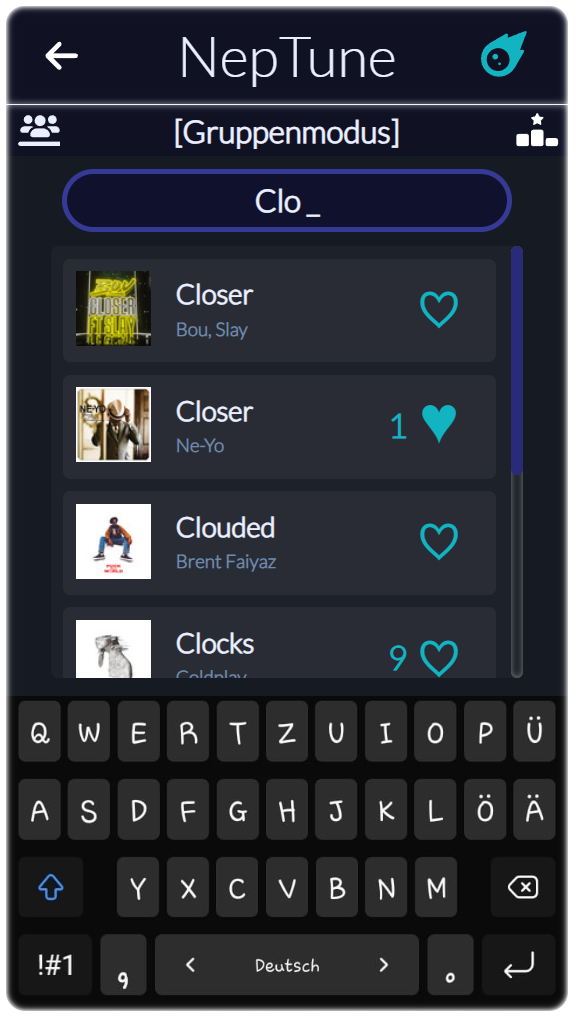
\includegraphics[width=0.9\textwidth]{LATEX/Pflichtenheft/GraphicDesigns/userSearchPage.png}
    \captionof{figure}{participantSearchView}
\end{minipage} 
\hfill
\begin{minipage}{0.5\textwidth}
    XXX
\end{minipage}

\textbf{Session-Info:}
\begin{itemize}
    \item Durch Klicken auf den Button Session-Info (der mit dem Gruppen-Icon) gelangt man in die sessionInfoView (REF).
\end{itemize}

\textbf{Statistiken:}
\begin{itemize}
    \item Durch Klicken auf den Button Session-Info (der mit dem Balken-Icon) gelangt man in die sessionStatsView (REF).
\end{itemize}

\textbf{Track-Eingabefeld:}
\begin{itemize}
    \item Eingabefeld für den Suchbegriff. Ändert sich der Eingabebegriff, wird die Track-Anzeige aktualisiert.
\end{itemize}

\textbf{Track-Anzeige:}
\begin{itemize}
    \item Grundsätzlich nicht klickbare (außer dem Track-Upvote-Button) Liste von Tracks, die dem eingegebenen Suchbegriff entsprechen. Jeder Track wird mit Cover, Titel, Interpret und der Anzahl der Upvotes angezeigt, sowie der Information, ob der User den Track geupvotet hat.
    \item Bei Full Participants wird dabei der gesamte Musikkatalog von Spotify durchsucht, um zum Suchbegriff passende Tracks zu finden, mit folgenden Einschränkungen:
    \begin{itemize}
        \item Im General Mode gibt es keine Einschränkungen.
        \item Im Artist Mode werden nur Tracks der vom Host bei Sessionerstellung (REF) definierten Artists angezeigt.
        \item Im Genre Mode werden nur Tracks der vom Host bei Sessionerstellung (REF) definierten Genres angezeigt.
        \item Im Playlist Mode werden nur Tracks der vom Host bei Sessionerstellung (REF) definierten Playlist angezeigt.
    \end{itemize}
    \item Bei Restricted Participants wird nur die Vorschlagsliste durchsucht, die Tracks mit mindestens einem Upvote enthält. Ausnahme ist der Playlist Mode, darin werden alle Tracks der Playlist durchsucht ohne Berücksichtigung der Upvotes.
\end{itemize}

\textbf{Track-Upvote:}
\begin{itemize}
    \item Durch Klicken des Track-Upvote-Buttons eines Tracks (der mit dem Herz) erhöht sich der Counter der Upvotes des Tracks und das Herz wird ausgefüllt. Der erste Upvote, also das erste Klicken auf einen Track ohne bisherige Upvotes, entspricht dem Vorschlagen eines Tracks.
    \item Durch erneutes Klicken des bereits geklickten Track-Upvote-Buttons eines Tracks verringert sich der Counter der Upvotes des Tracks und das Herz wird leer. Der Button kehrt in seinen ursprünglichen Zustand zurück.
\end{itemize}

\textbf{Zurück-Button:}
\begin{itemize}
    \item Durch Klicken des Zurück-Buttons gelangt man in die  \hyperlink{sessionVoteView}{sessionVoteView}.
\end{itemize}

\newpage

\subsection{Moduswahl für den Host (hostModeSelectView)}
\label{sec:Benutzeroberfläche:joinSessionView}


\begin{minipage}{0.5\textwidth}
    \hypertarget{hostModeSelectView}{}
    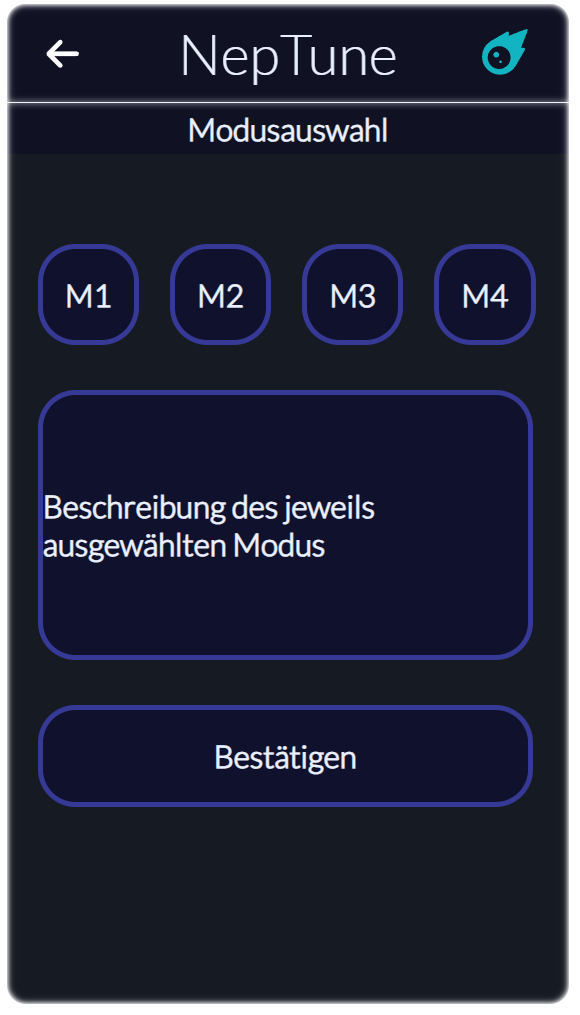
\includegraphics[width=0.9\textwidth]{LATEX/Pflichtenheft/GraphicDesigns/hostModusSelectPage.png}
    \captionof{figure}{hostModeSelectView}
\end{minipage} 
\hfill
\begin{minipage}{0.5\textwidth}
    XXX
\end{minipage}

\textbf{Modus-Buttons:}
\begin{itemize}
    \item Es stehen vier Modus-Buttons zur Verfügung:
    \begin{itemize}
        \item Der erste Button ist für den General Mode (REF Use-Case-Diag.)
        \item Der zweite Button ist für den Artist Mode (REF Use-Case-Diag.)
        \item Der dritte Button ist für den Genre Mode (REF Use-Case-Diag.)
        \item Der vierte Button ist für den Playlist Mode (REF Use-Case-Diag.)
    \end{itemize}
    \item Durch Klicken auf einen der vier Modus-Buttons wird dieser markiert. Es kann stets nur ein Modus-Button markiert sein. Zu Beginn ist kein Button markiert. Der Modus des markierten Buttons ist angewählt.
\end{itemize}

\textbf{Modus-Info-Anzeige:}
\begin{itemize}
    \item Die nicht klickbare Anzeige beinhaltet eine kurze Beschreibung des angewählten Modus.
\end{itemize}

\textbf{Modus bestätigen:}
\begin{itemize}
    \item Der Modus-Bestätigen-Button ist zunächst verblasst und nicht klickbar. Er wird erst klickbar, nachdem ein Modus angewählt wurde.
    \item Durch Klicken des Modus-Bestätigen-Buttons wird der angewählte Modus ausgewählt und der Host gelangt in die EinstellungsView (REF).
\end{itemize}

\textbf{Zurück-Button:}
\begin{itemize}
    \item Durch Klicken des Zurück-Buttons gelangt man in die  \hyperlink{startView}{startView}.
\end{itemize}

\newpage

TODO: Ab hier weitermachen im obigen Format, also einfach copy paste und ausfüllen...

\begin{figure}
    \hypertarget{hostModusSettingsPage}{}
    \begin{minipage}[t]{7 cm}
        \vspace{-1.5ex}
        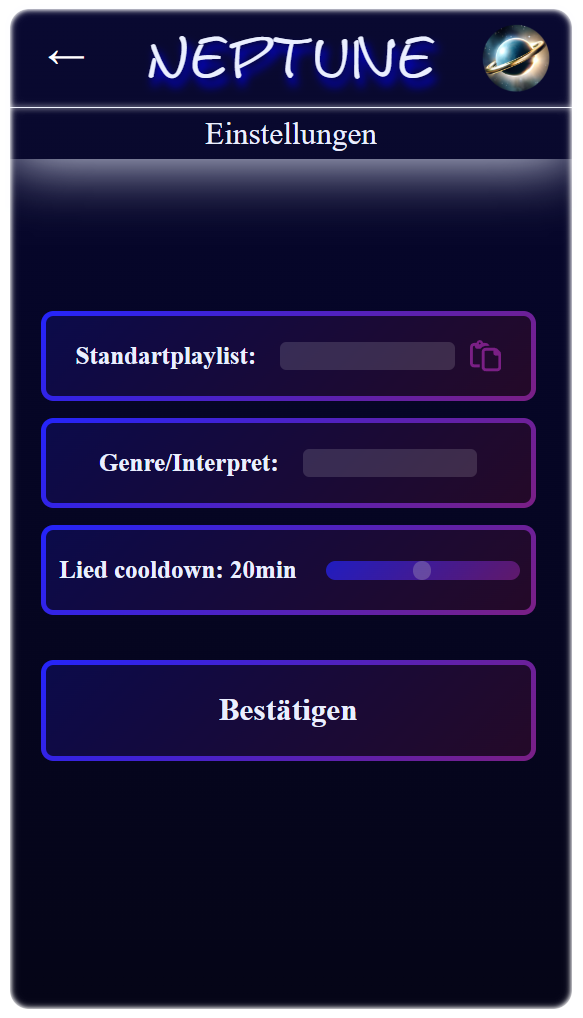
\includegraphics[width=7cm]{LATEX/Pflichtenheft/GraphicDesigns/hostModusSettingsPage.png}
        \caption{hostModusSettingsPage}
    \end{minipage}
    \hspace{1cm}
    \begin{minipage}[t]{7 cm}
        \vspace{1cm}
        In den Host Einstellungen kann man mit dem Einfügen eines Spotifyplaylistlinkes eine Standartplaylist hinterlegen.
        In der Genre/Artist Feld kann man die Genre und Artistbeschränkungen auswählen \textit{(Todo wie)}
    \end{minipage}
\end{figure}

\begin{figure}
    \hypertarget{hostControlPage}{}
    \begin{minipage}[t]{7 cm}
        \vspace{-1.5ex}
        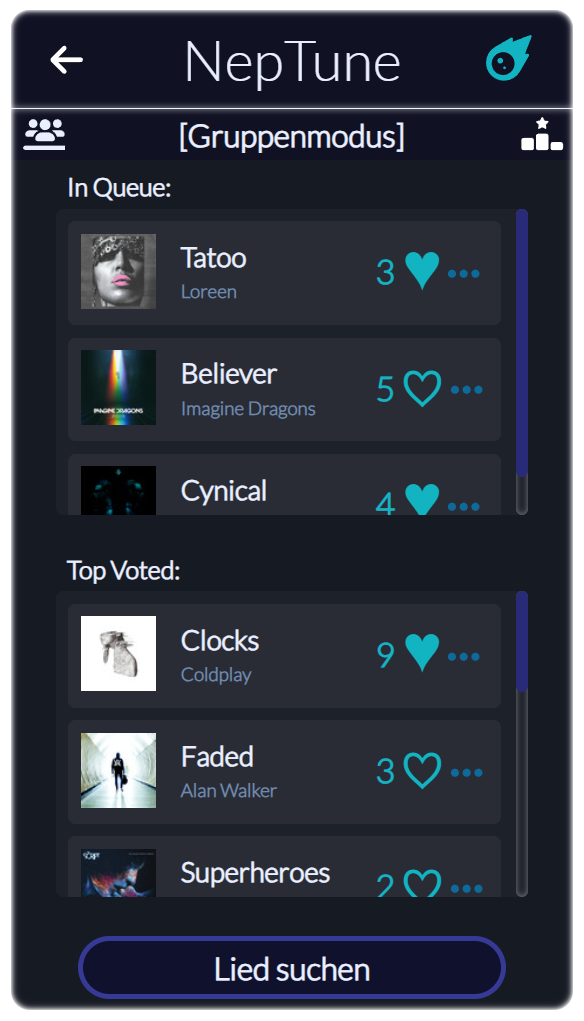
\includegraphics[width=7cm]{LATEX/Pflichtenheft/GraphicDesigns/hostControlPage.png}
        \caption{hostControlPage}
    \end{minipage}
    \hspace{1cm}
    \begin{minipage}[t]{7 cm}
        \vspace{1cm}
        In der HostControlPage kann der Host die Queue in Spotify einsehen. Genau wie ein Participant kann er hier Upvotes auf Tracks verteilen und wieder entfernen. Zudem kann der Host durch drücken auf die drei Punkte eines Tracks weitere Einstellung vornehmen. Zu diesen gehören das Hinzufügen und Entfernen eines Tracks zur Queue, sowie das Sperren und Entsperren von Tracks. Gesperrte Tracks können keine Upvotes erhalten und werden nicht abgespielt.
    \end{minipage}
\end{figure}

\begin{figure}
    \hypertarget{hostSearchPage}{}
    \begin{minipage}[t]{7 cm}
        \vspace{-1.5ex}
        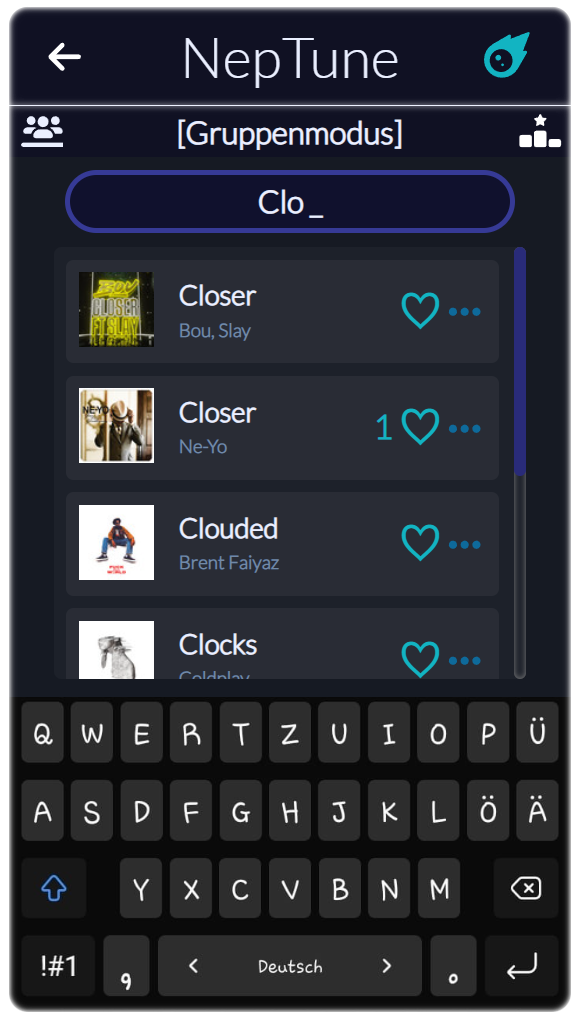
\includegraphics[width=7cm]{LATEX/Pflichtenheft/GraphicDesigns/hostSearchPage.png}
        \caption{hostSearchPage}
    \end{minipage}
    \hspace{1cm}
    \begin{minipage}[t]{7 cm}
        \vspace{1cm}
        TODO
    \end{minipage}
\end{figure}

\begin{figure}
    \hypertarget{shareLinkPopUpPage}{}
    \begin{minipage}[t]{7 cm}
        \vspace{-1.5ex}
        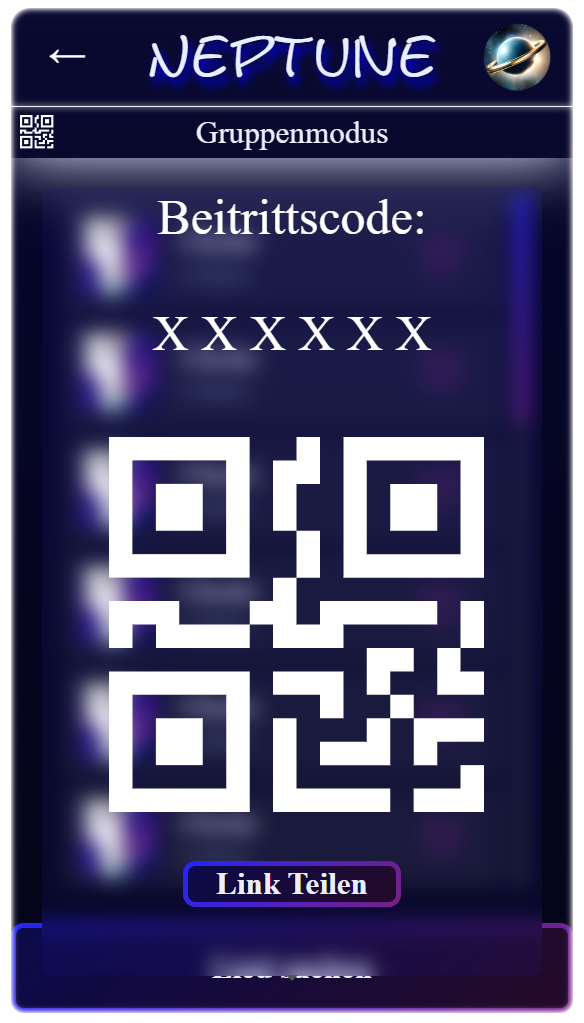
\includegraphics[width=7cm]{LATEX/Pflichtenheft/GraphicDesigns/shareLinkPopUpPage.png}
        \caption{shareLinkPopUpPage}
    \end{minipage}
    \hspace{1cm}
    \begin{minipage}[t]{7 cm}
        \vspace{1cm}
        Die shareLinkPopUpPage stellt für den Host einer Session in gebündelter Form Möglichkeiten zur Verfügung,  User als Participants zu der entsprechenden Session einzuladen. Primär stehen hierfür ein der Session eindeutig zugeordneter, sechstelliger Code aus Ganzzahlen sowie ein analog der Session zugeordneter Beitrittslink zur Verfügung. Für den Beitrittslink ist in der Anzeige ein Button enthalten, mithilfe dessen der Link geteilt werden kann. Für das Teilen wird hierbei die von Android bereitgestellte Schnittfläche verwendet. Darüber hinaus soll als Alternative gleichzeitig auch ein analog funktionierender QR-Code zur Verfügung stehen, welcher in dieser Ansicht mit angezeigt wird. Zusätzlich werden in dieser Anzeige der Bezeichner des Gruppenmodus der Session sowie gegebenenfalls Informationen über Modusseitige Einschränkungen hinsichtlich Genres und Artists angezeigt. Durch Auswahl des "Zurück
 Buttons (symbolisiert durch Pfeil) gelangt man zur zuvor angezeigten Ansicht zurück. Durch Auswahl des "X"-Buttons lässt sich diese Anzeige schließen und man gelangt zur \textit{(uv)-}Ansicht. \textit{(TODO: ENTSPRECHENDE ANSICHT DAZU SCHREIBEN!)}
 \end{minipage}
\end{figure}

\begin{figure}
    \hypertarget{statisticsPopUpPage}{}
    \begin{minipage}[t]{7 cm}
        \vspace{-1.5ex}
        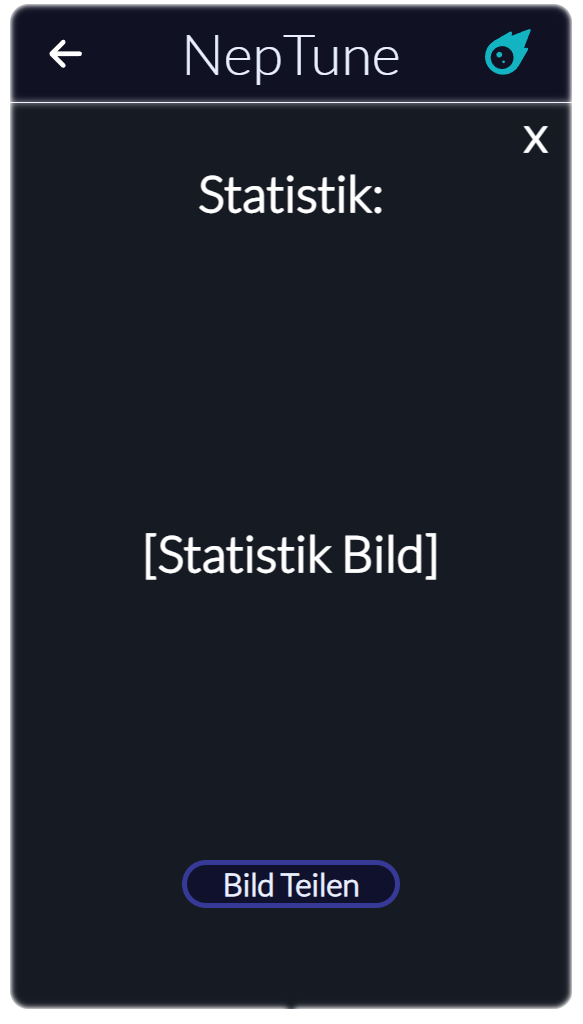
\includegraphics[width=7cm]{LATEX/Pflichtenheft/GraphicDesigns/statisticsPopUpPage.png}
        \caption{statisticsPopUpPage}
    \end{minipage}
    \hspace{1cm}
    \begin{minipage}[t]{7 cm}
        \vspace{1cm}
        TODO
    \end{minipage}
\end{figure}


% show subsections in contents
\addtocontents{toc}{\protect\setcounter{tocdepth}{2}}
\chapter{Anwendungsfälle}
\label{chap:Anwendungsfälle}

In diesem Kapitel werden einige Anwendungsfälle der App mithilfe von Use Case Diagrammen anschaulich gemacht. Diese beschreiben das Starten einer Session, sowie die einzelnen Modi der App.

\section{Session erstellen}
\label{sec:Anwendungsfälle:Session erstellen}

\begin{figure}[h]
   \hypertarget{Anwendungsfaelle}{}
    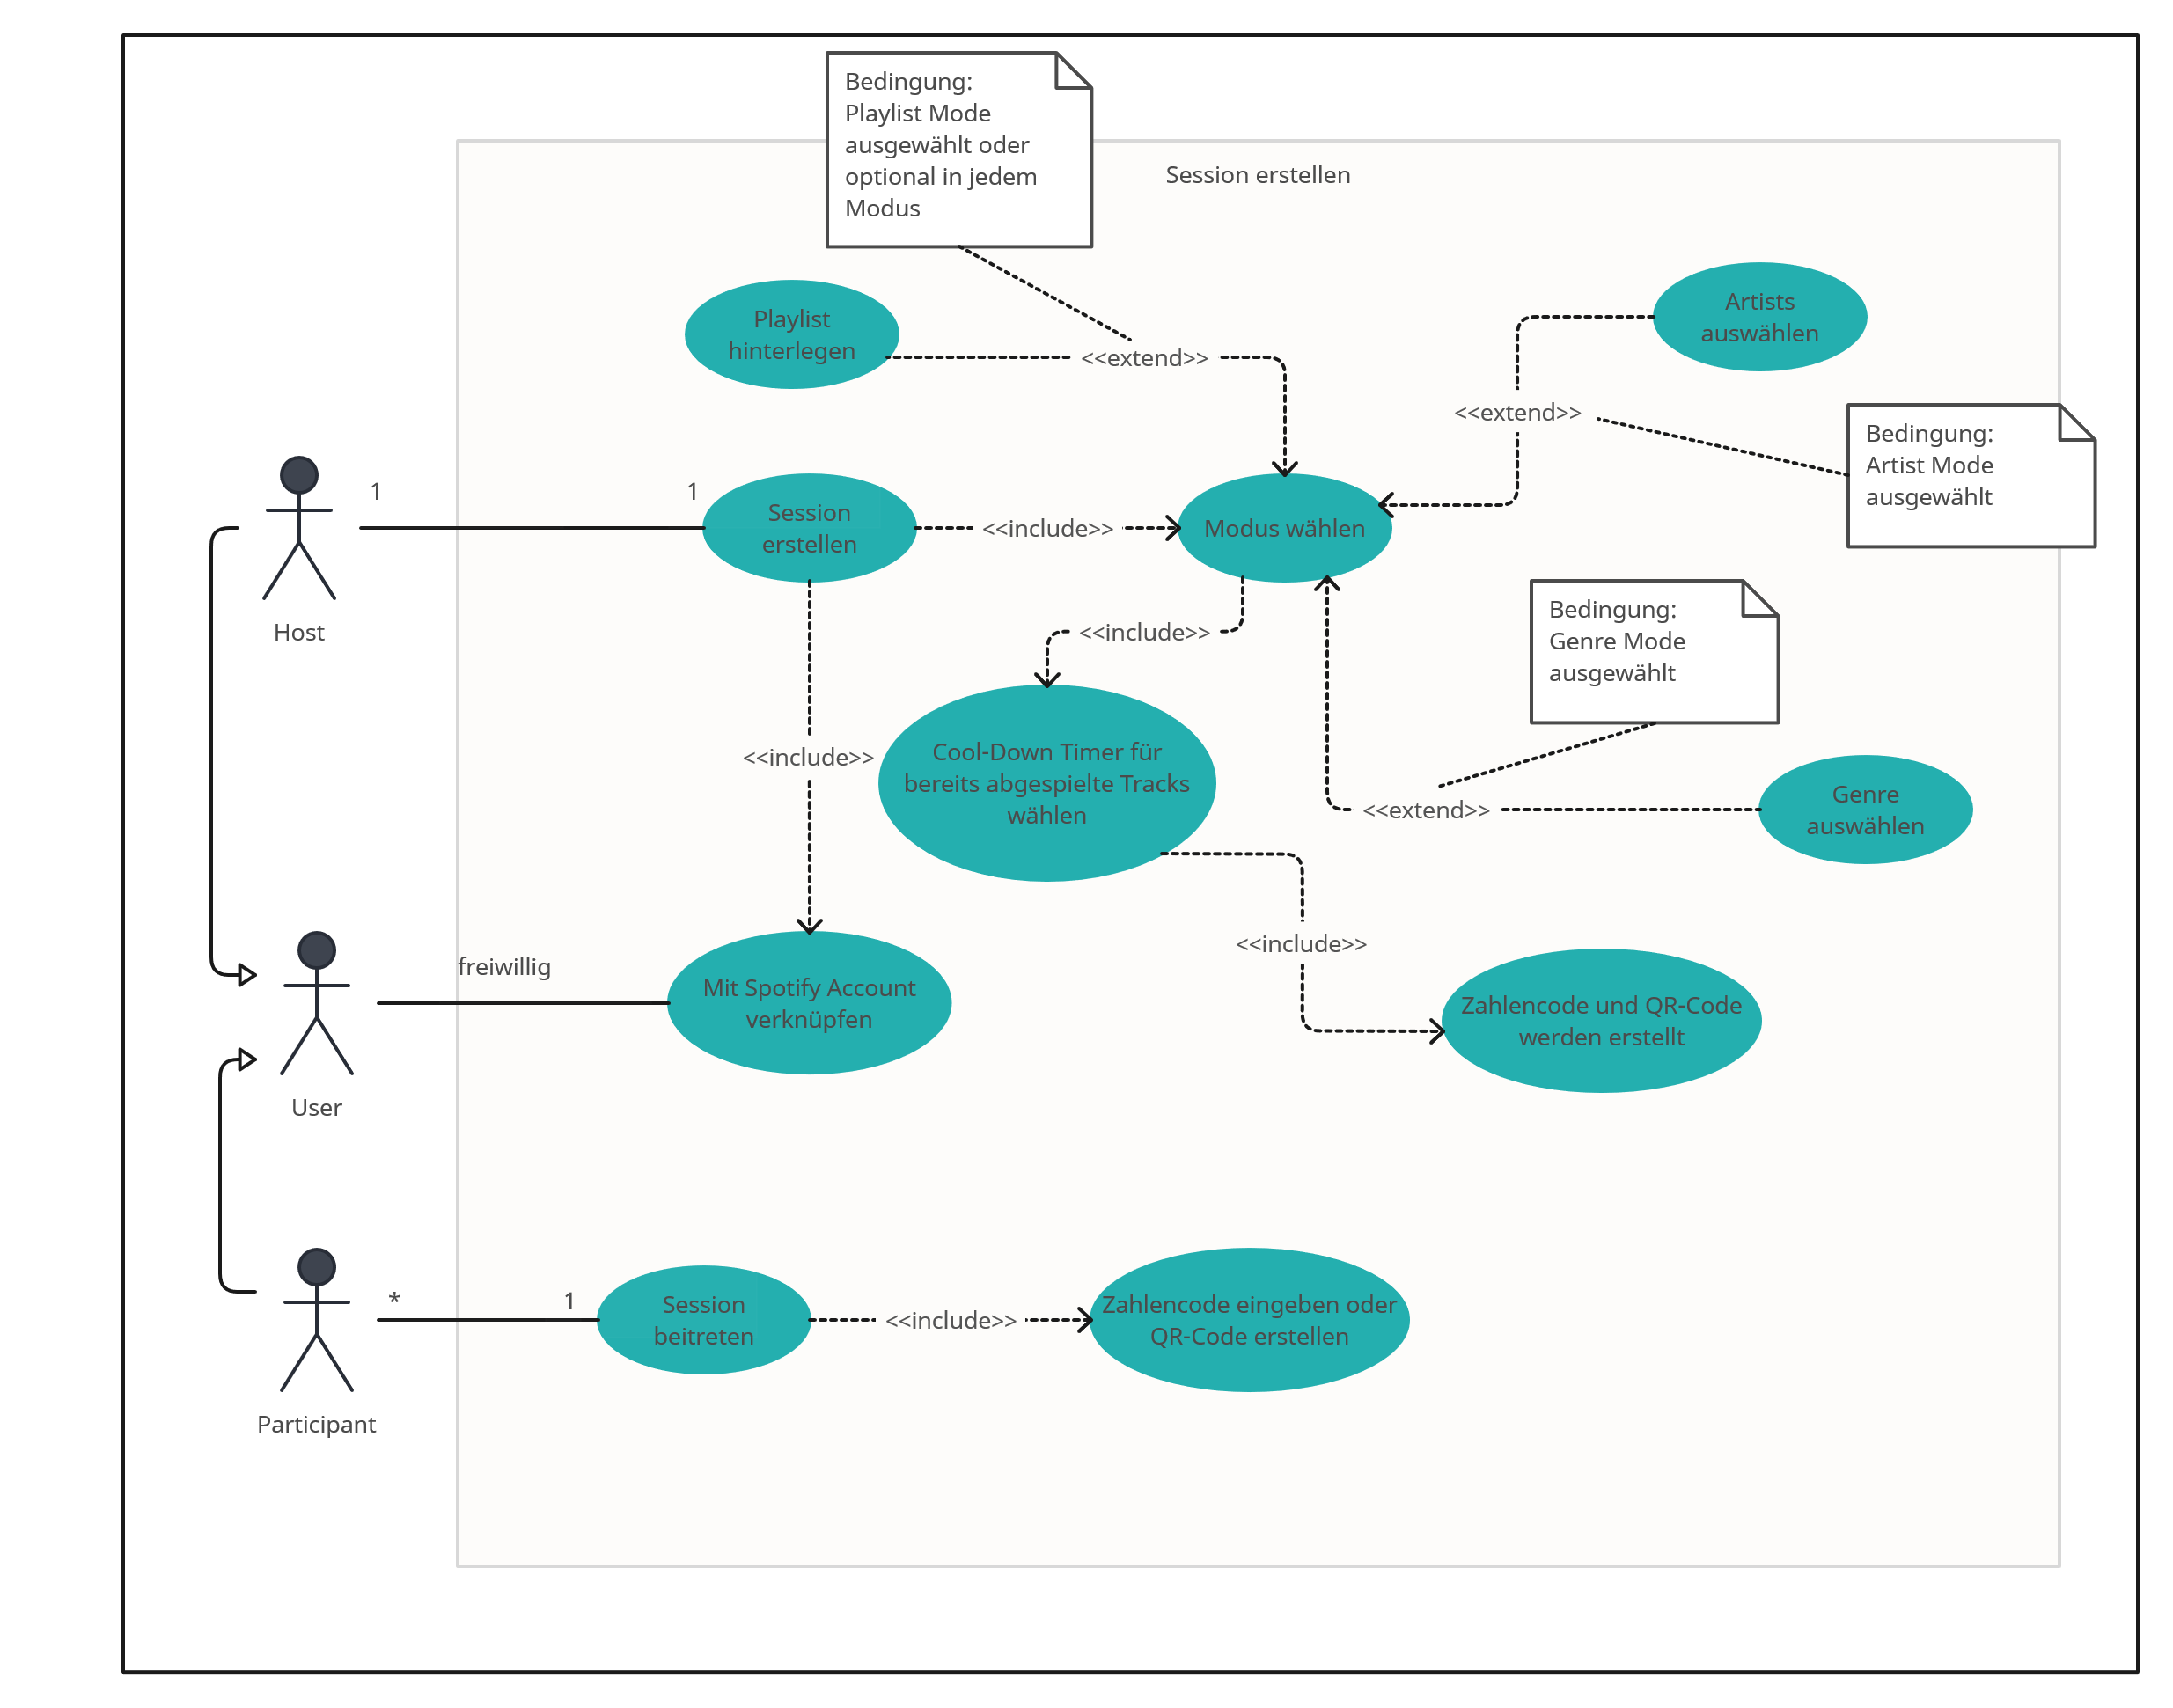
\includegraphics[width = 16cm]{LATEX/Pflichtenheft/GraphicDesigns/Use Case Session erstellen.png}
    \caption{Session erstellen}
    \label{fig:Use Case App Start}
\end{figure}

\newpage

\section{General Mode}
\label{sec:Anwendungsfälle:General Mode}

\begin{figure}[h]
    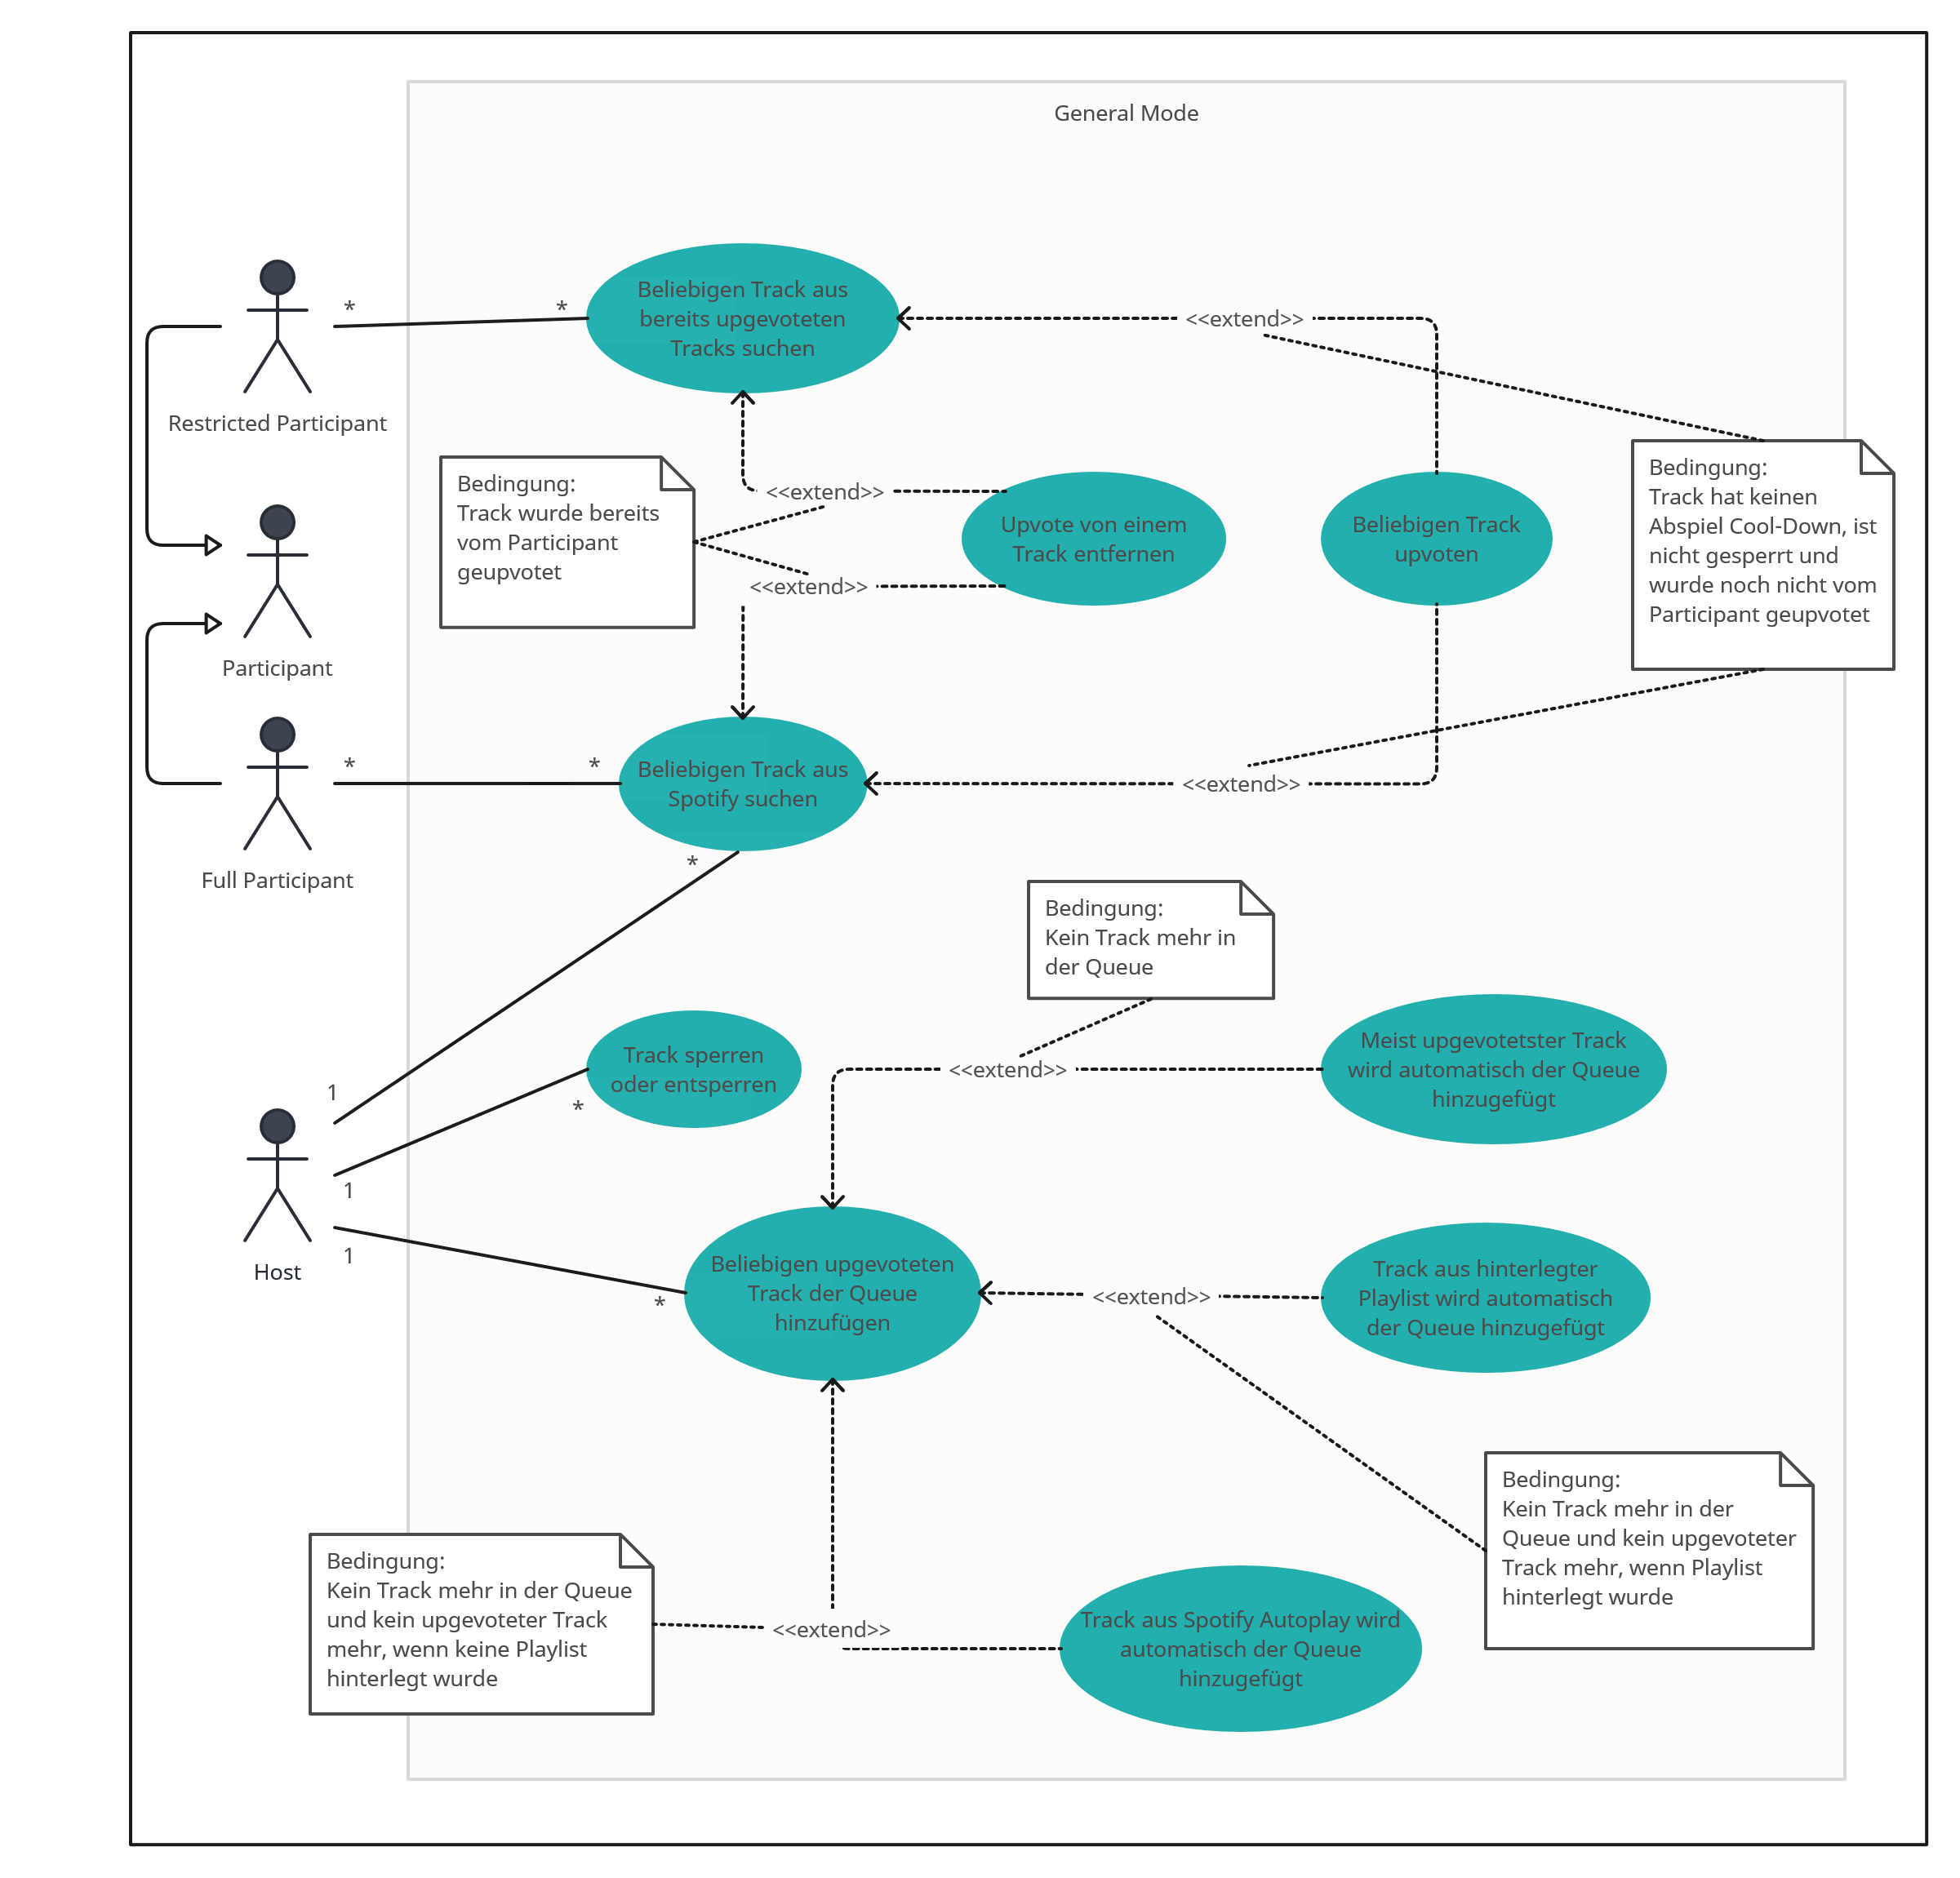
\includegraphics[width = 16cm]{LATEX/Pflichtenheft/GraphicDesigns/Use Case General Mode.png}
    \caption{General Mode}
    \label{fig:Use Case General Mode}
\end{figure}

\newpage

\section{Artist Mode}
\label{sec:Anwendungsfälle:Artist Mode}

\begin{figure}[h]
    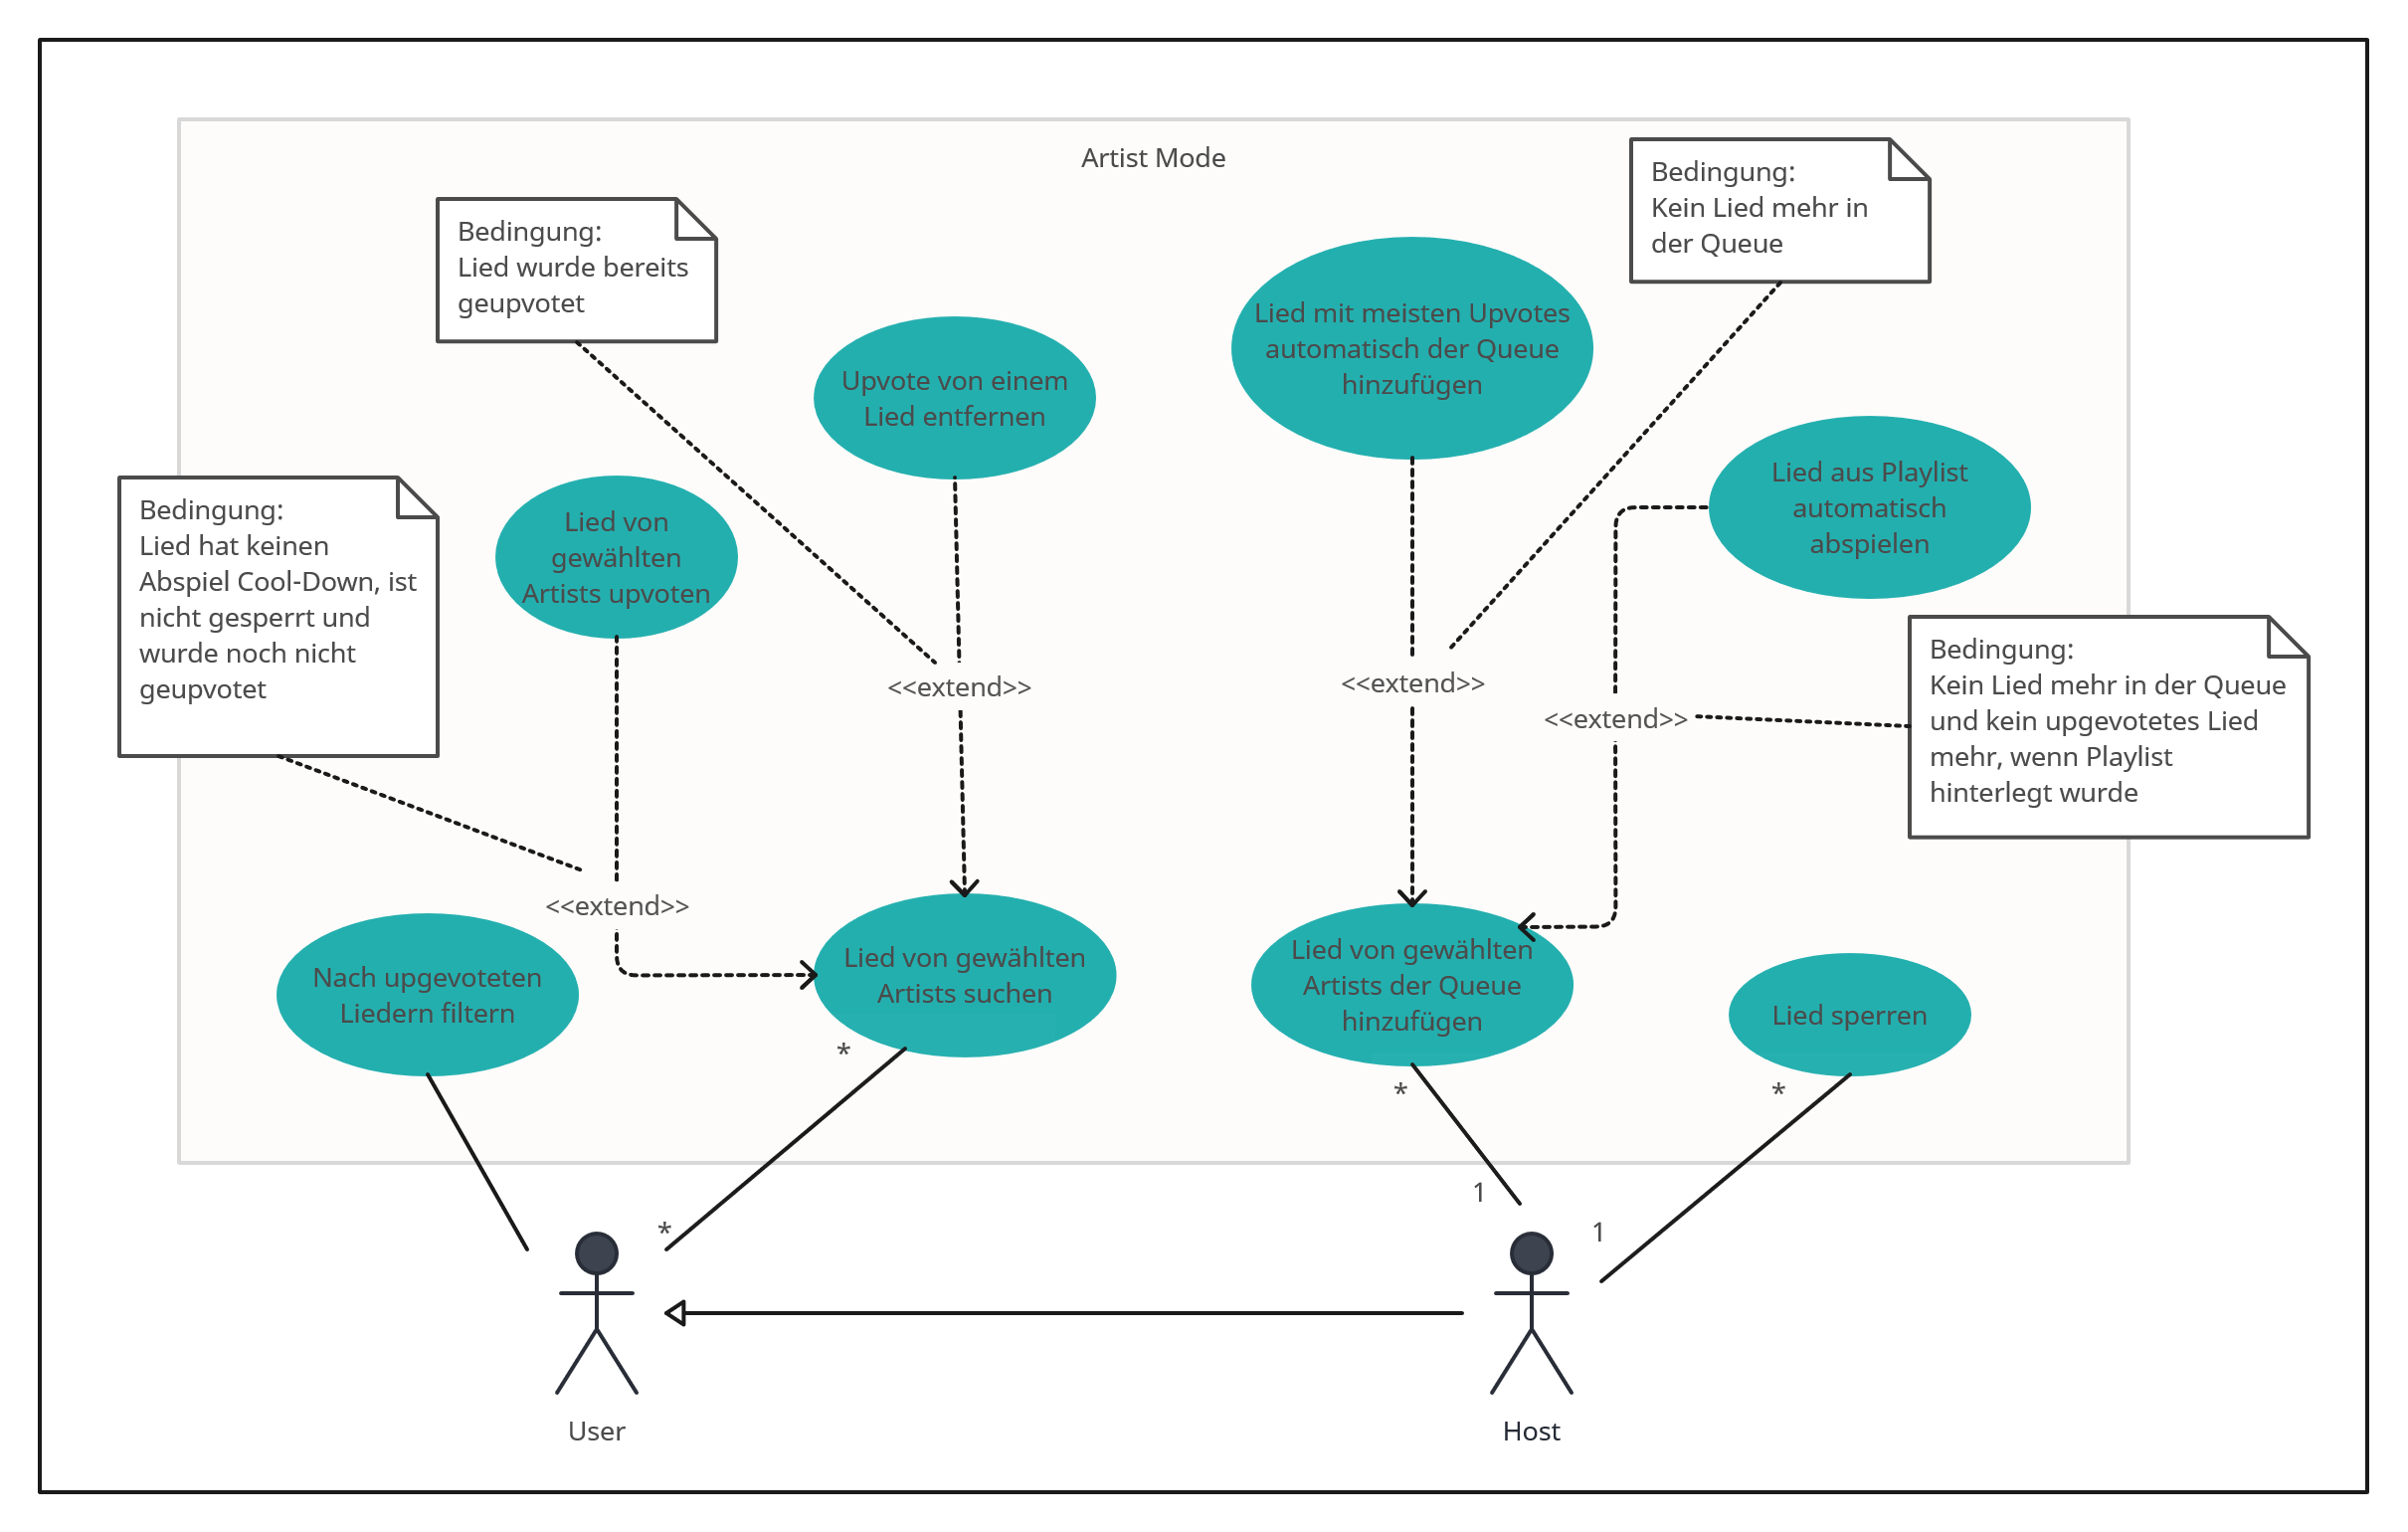
\includegraphics[width = 16cm]{LATEX/Pflichtenheft/GraphicDesigns/Use Case Artist Mode.png}
    \caption{Artist Mode}
    \label{fig:Use Case Artist Mode}
\end{figure}

\newpage

\section{Genre Mode}
\label{sec:Anwendungsfälle:Genre Mode}

\begin{figure}[h]
    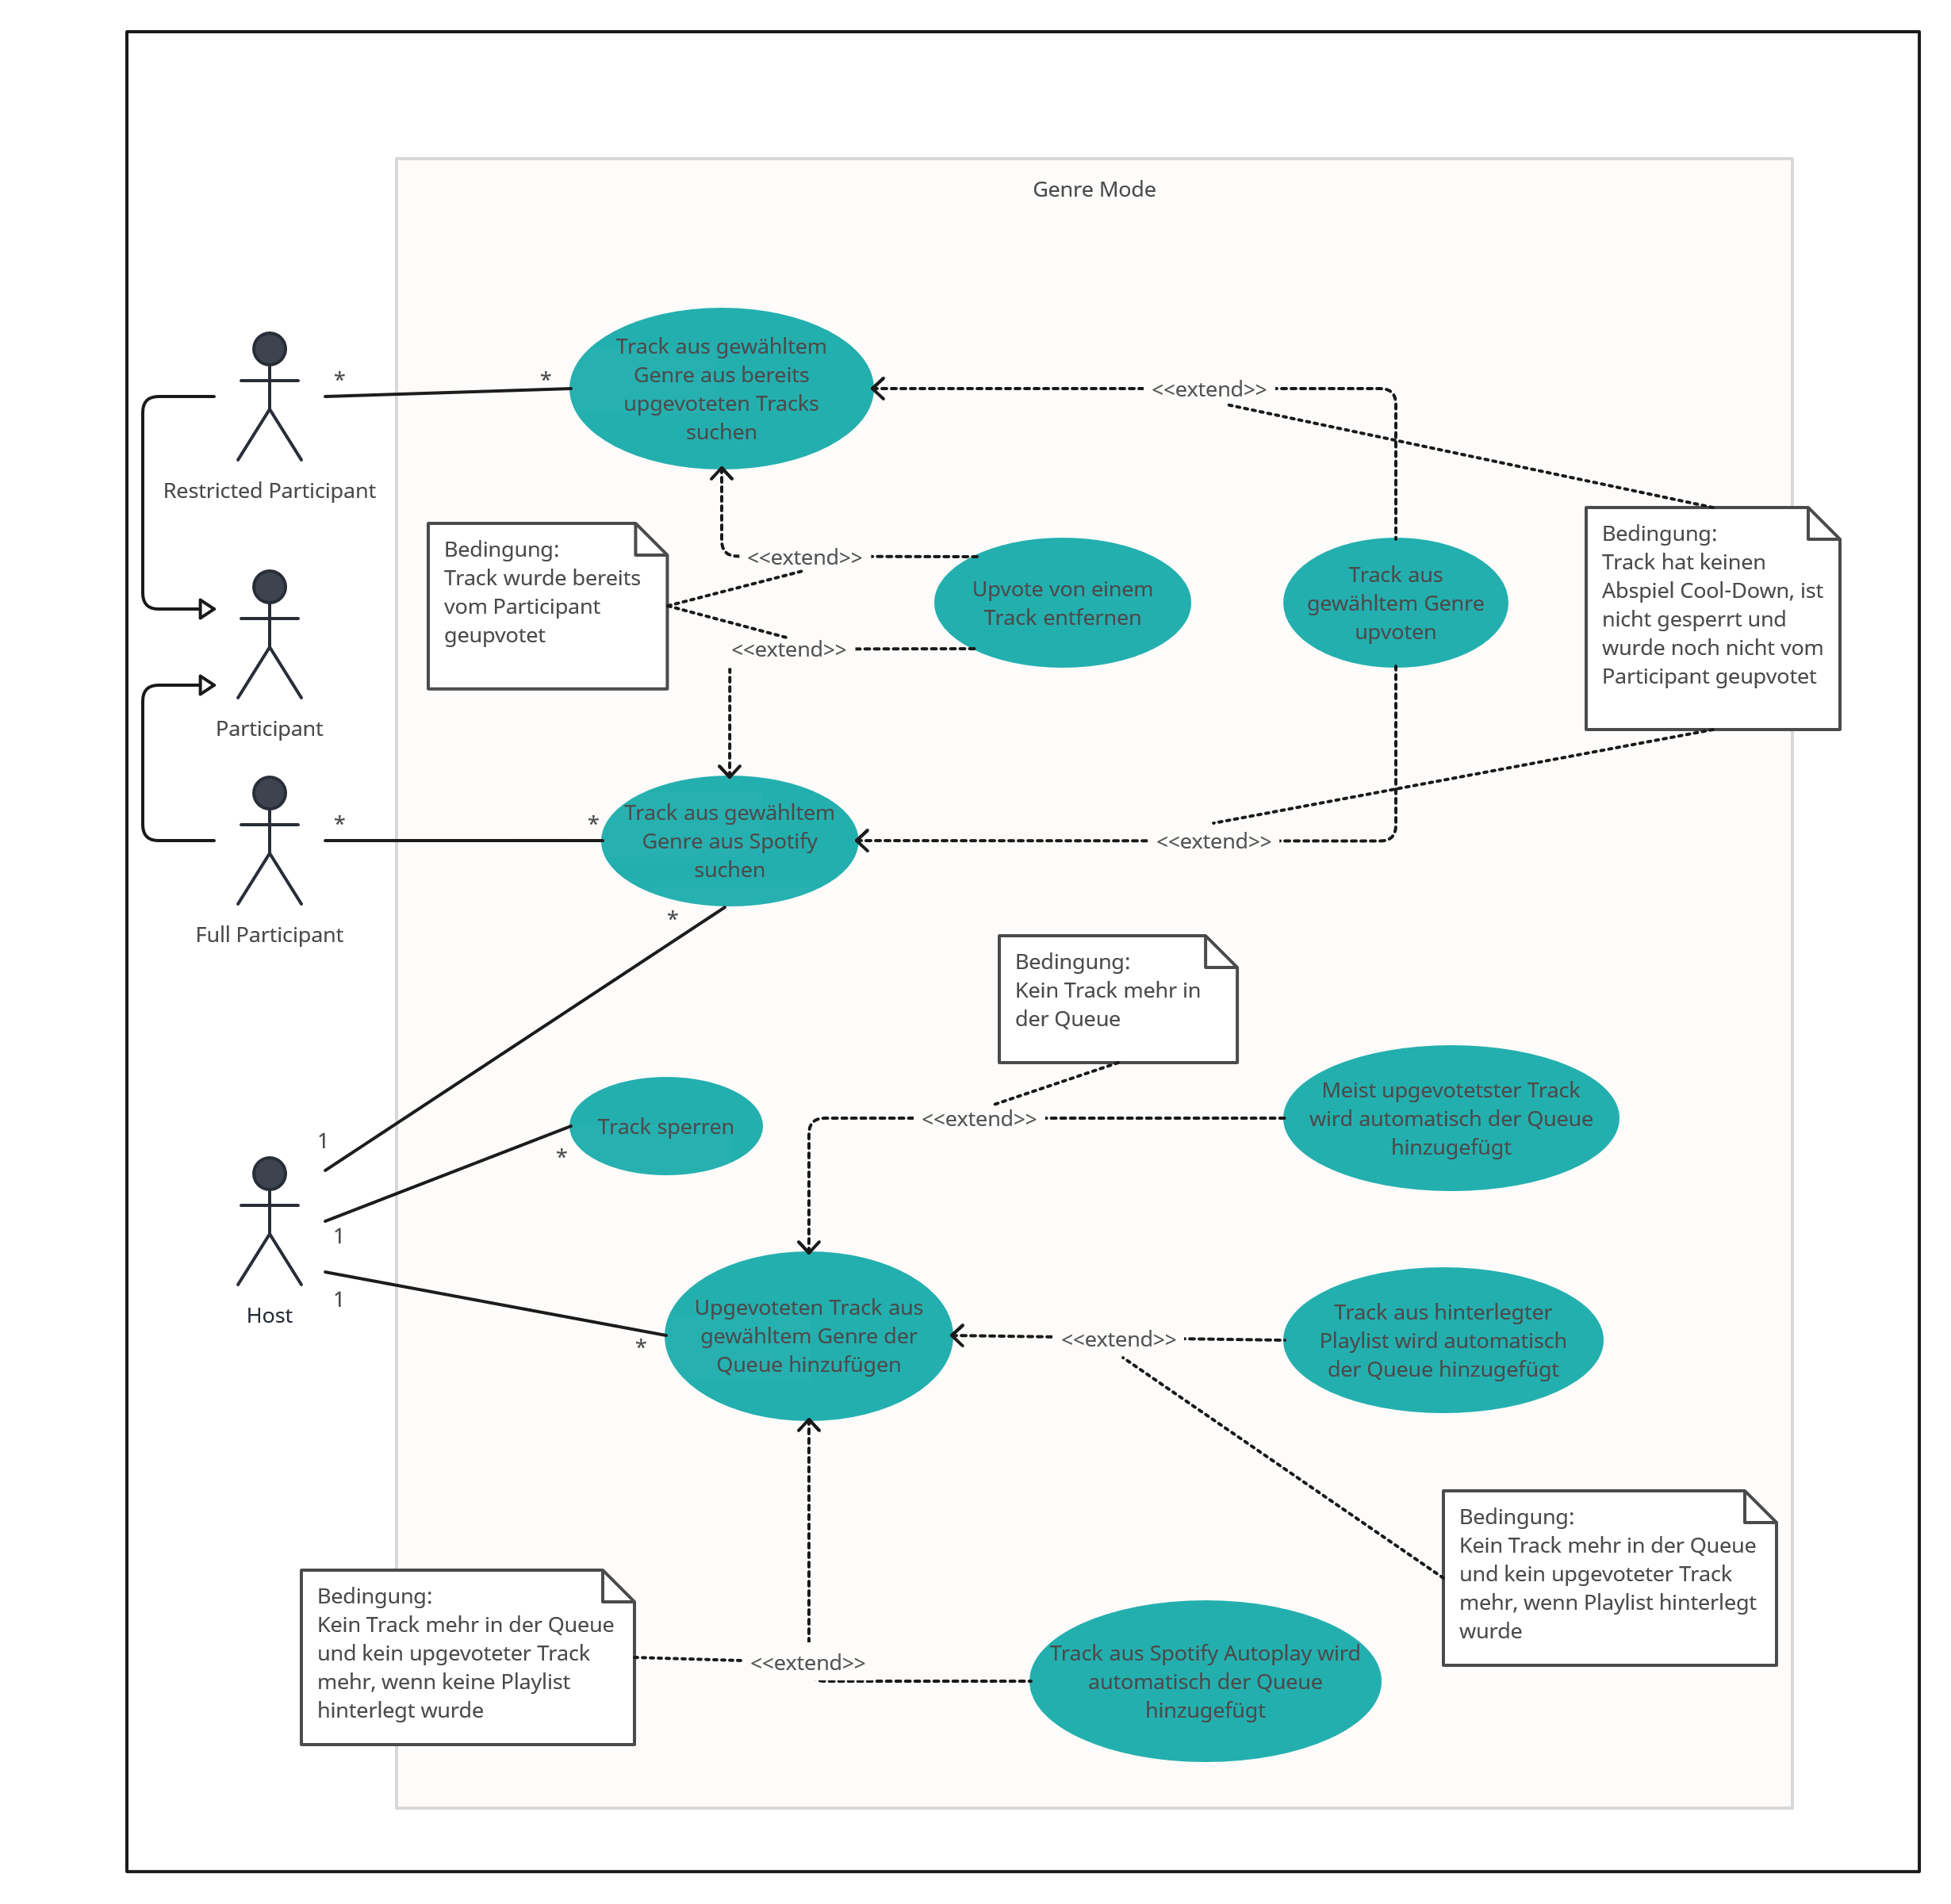
\includegraphics[width = 16cm]{LATEX/Pflichtenheft/GraphicDesigns/Use Case Genre Mode.png}
    \caption{Genre Mode}
    \label{fig:Use Case Genre Mode}
\end{figure}

\newpage

\section{Playlist Mode}
\label{sec:Anwendungsfälle:Playlist Mode}

\begin{figure}[h]
    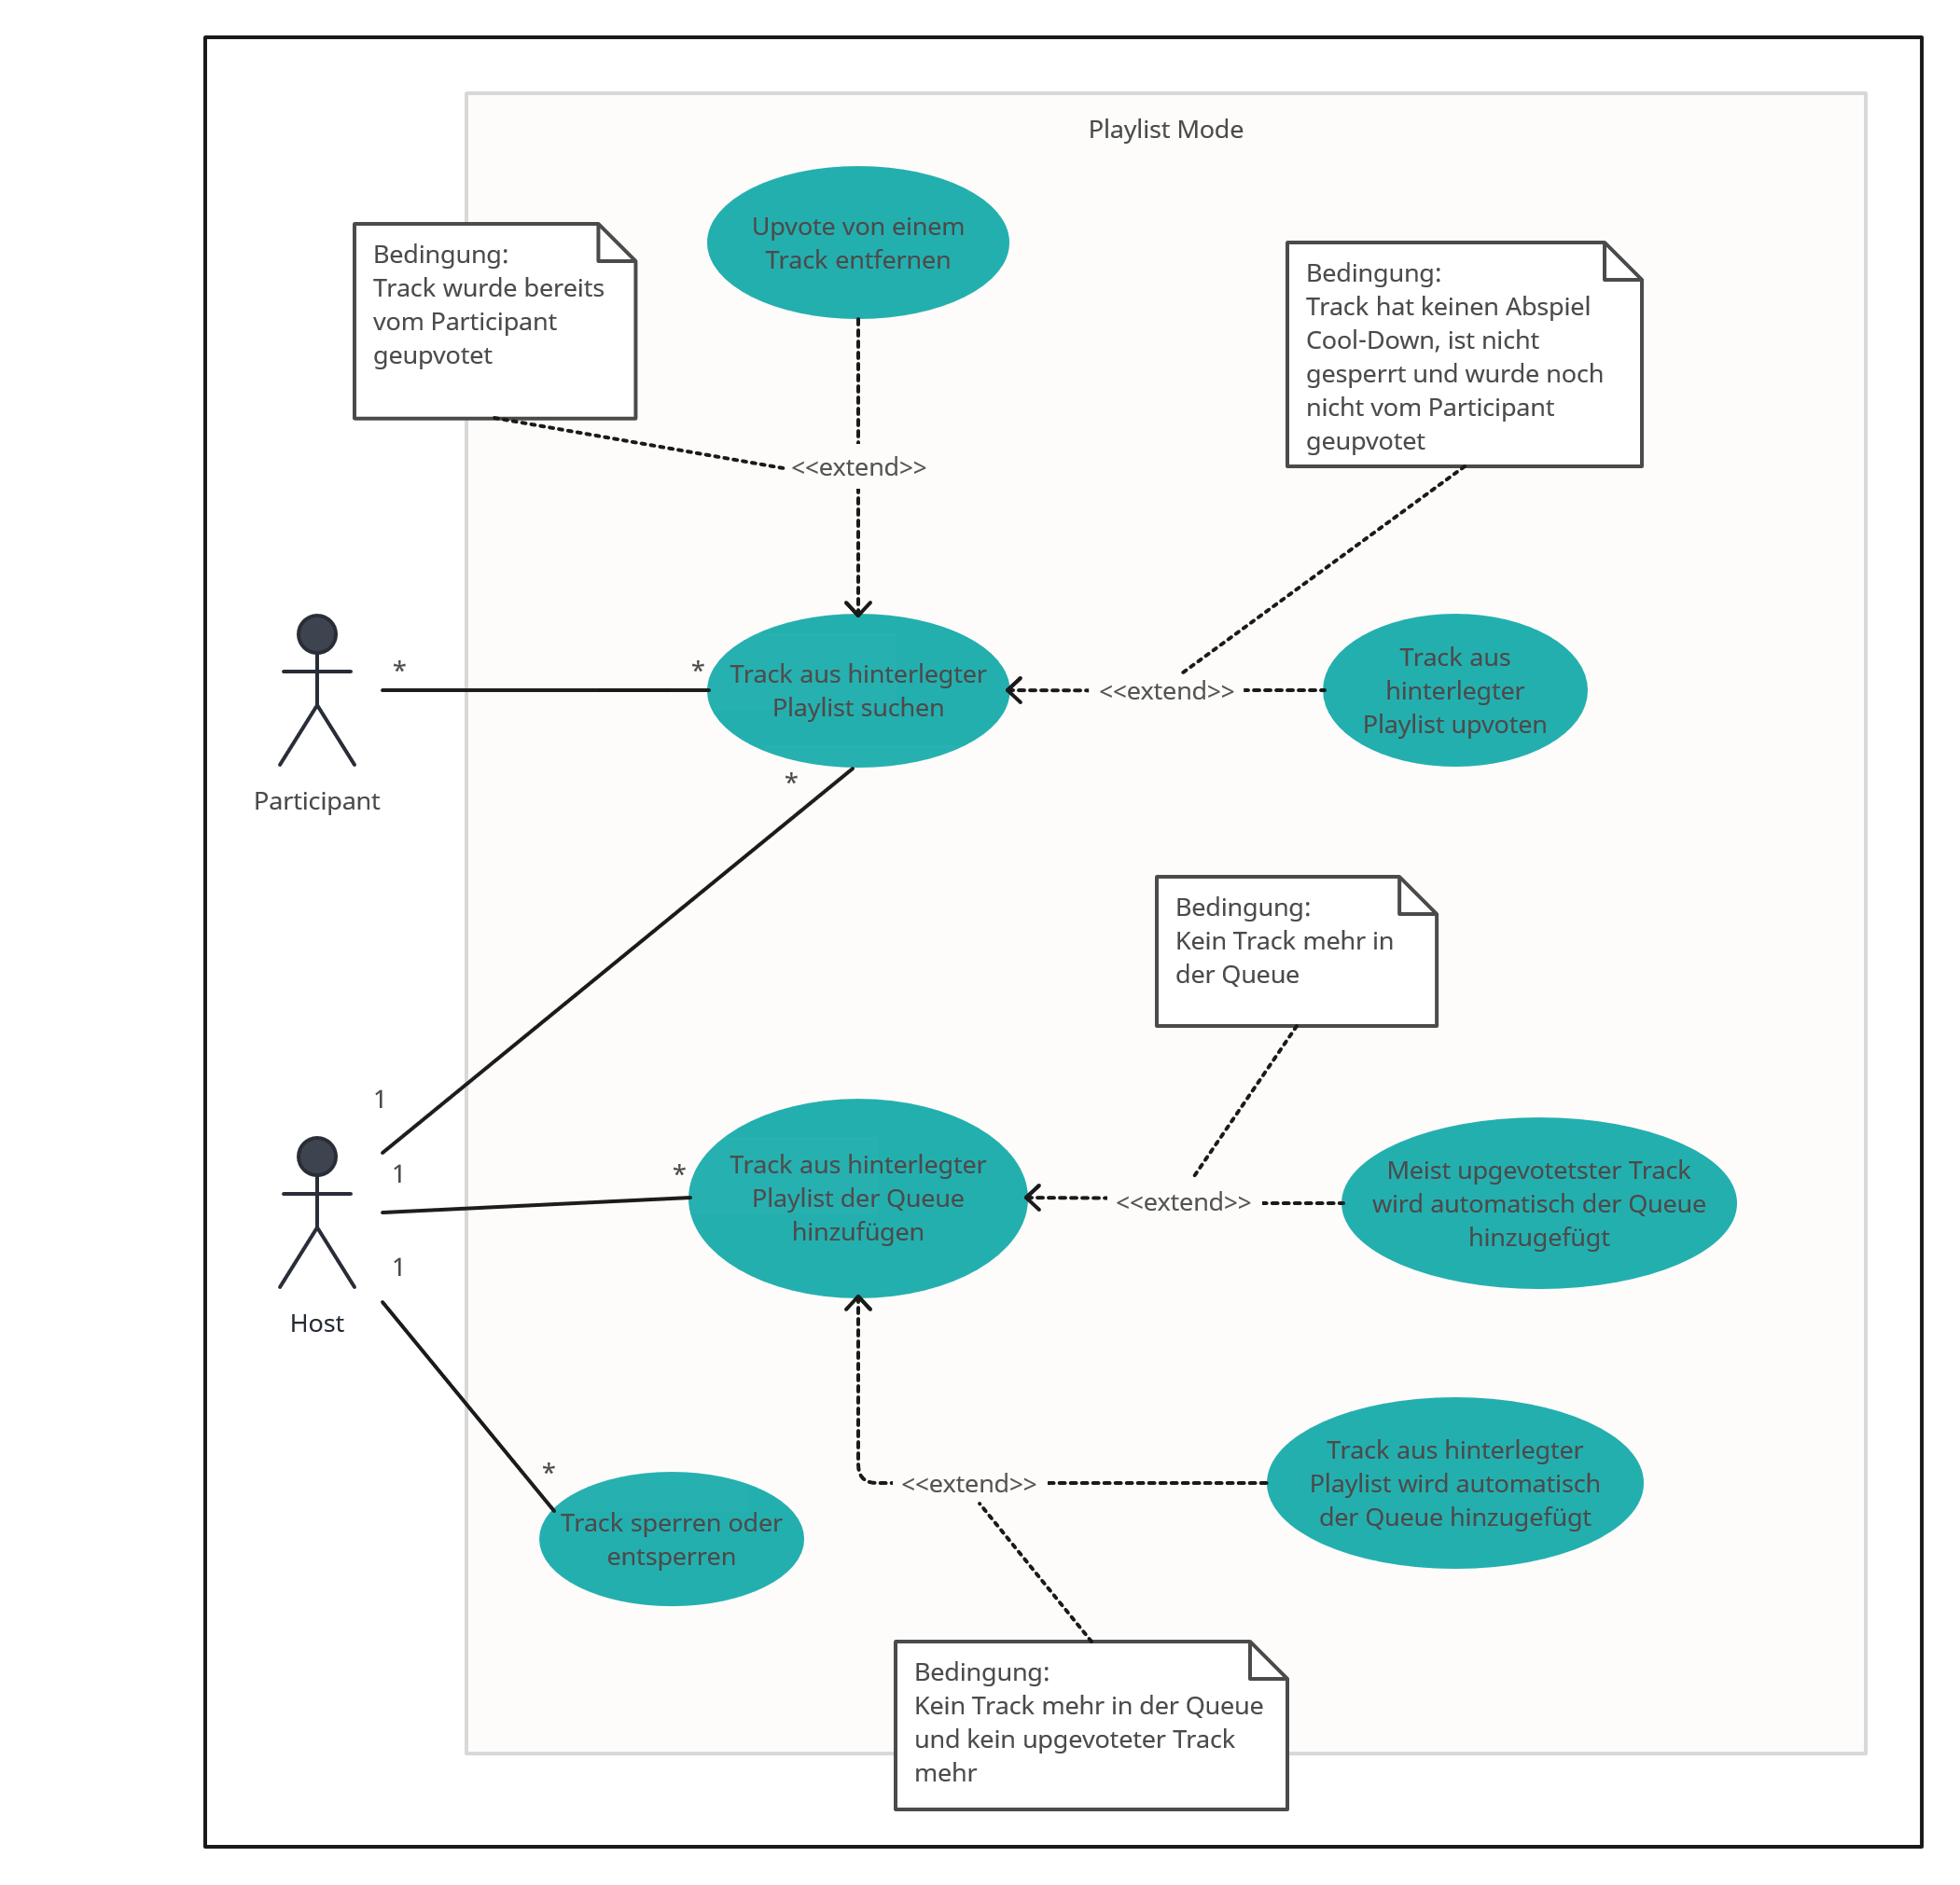
\includegraphics[width = 16cm]{LATEX/Pflichtenheft/GraphicDesigns/Use Case Playlist Mode.png}
    \caption{Playlist Mode}
    \label{fig:Use Case Playlist Mode}
\end{figure}



\chapter{Testfälle und -szenarien}
\label{chap:Tests}

In diesem Kapitel werden alle Testfälle und -szenarien definiert, die durch einen oder mehrere Benutzer des Produkts durchgeführt werden können. Die hier definierten Testfälle sollen deshalb explizit keine technischen Funktionalitäten testen, die ausreichend detailliert erst während der Entwurfsphase festgelegt werden. Solche technischen Funktionalitäten werden durch Unittests abgedeckt, die während der Entwurfs- und Implementierungsphase entworfen und implementiert werden.

\section{Testfälle}
\label{sec:Tests:Testfälle}

TODO: Liste wegmachen und einfach die funktionalen Anforderungen durchnummerieren. Das sind dann einfach alle Testfälle.

Testfälle sind Tests zu aus Usersicht atomaren Vorgängen. Jeder Testfall bezieht sich also auf eine einzelne atomare Usereingabe. Eine solche Usereingabe besteht entweder aus einem einzelnen Touch-Eingabe oder einer inhaltlich sehr stark zusammenhängenden Folge von Touch-Eingaben, die als atomar betrachtet wird. Falls ein Testfall nur für eine bestimmte Gruppe von Usern ausführbar ist, steht das in Klammern hinter dem Testfall mit folgenden verwendeten Abkürzungen: Host (H), Participant (P), Full Participant (FP) und Restricted Participant (RP).

\begin{enumerate}
    \item Starten und Laden der App
    \item Verlassen der App
    \item Beenden der App
    \item Beginnen des Sessionbeitrittsvorgangs
    \item Verlassen des Sessionbeitrittsvorgangs
    \item Eingabe des Zugangscodes zum Sessionbeitritt
    \item Bestätigung des Zugangscodes zum Sessionbeitritt
    \item Verlassen der Session (P)
    \item Upvote für einen Track
    \item Entfernen des Upvote von einem Track
    \item Öffnen der Tracksuche (H, FP)
    \item Verlassen der Tracksuche (H, FP)
    \item Suchen eines Tracks (FP)
    \item Vorschlagen eines Track durch Upvote (FP)
    \item Beginnen der Sessionerstellung (H)
    \item Verlassen der Sessionerstellung in der Modus-Wahl (H)
    \item Wahl des Modus (H)
    \item Zurückgehen in der Sessionerstellung von den Modus-Details zur Modus-Wahl (H)
    \item Auswählen der Details des Modus (H)
    \begin{itemize}
        \item Auswählen der Artists / der Genres / der Playlist (je nach Modus)
        \item Einstellen des Cool-Downs, wann ein Lied erneut vorgeschlagen werden kann
    \end{itemize}
    \item Bestätigung der Details des Modus (H)
    \item Löschen der Session (H)
    \item Löschen eines Tracks aus der Queue (H)
    \item Einfügen eines Tracks in die Queue aus der Tracksuche (H)
    \item Einfügen eines Tracks in die Queue aus der Vorschlagsliste (H)
    \item Ändern der Reihenfolge der Queue durch Drag and Drop (H)
    \item Löschen eines Tracks aus der Vorschlagsliste (H)
    \item Sperren eines Tracks (H) (Machen wir das überhaupt ???)
\end{enumerate}

\section{Grundlegende Testszenarien}
\label{sec:Tests:GrundlegendeTestszenarien}
% do not show subsections in contents
\addtocontents{toc}{\protect\setcounter{tocdepth}{1}}

Grundlegende Testszenarien sind eine überschaubare und besonders essentielle Folge von atomaren Testfällen, die eine Benutzerinteraktion durchspielen. Sie setzen sich aus Testfällen oder bereits zuvor definierten grundlegenden Testszenarien zusammen.

\subsection{Grundlegendes Testszenario 1 (G1): Erstellen einer Session}
\label{subsec:Tests:GrundlegendeTestszenarien:G1}
Ein User erstellt eine Session mit einem bestimmten Modus und wird so zu ihrem Host.
\begin{itemize}
    \item Starten und Laden der App
    \item Beginnen der Sessionerstellung
    \item Wahl des Modus
    \item Auswählen der Details des Modus
    \item Bestätigung der Details des Modus
\end{itemize}


\subsection{Grundlegendes Testszenario 2 (G2): Beitritt einer Session als Full Participant}
\label{subsec:Tests:GrundlegendeTestszenarien:G2}
Ein User, tritt als Full Participant einer Session mit einem bestimmten Modus bei, die von einem anderen User als Host erstellt wurde.
Dazu muss bereits G1 (\ref{subsec:Tests:GrundlegendeTestszenarien:G1}) abgelaufen sein.
\begin{itemize}
    \item Starten und Laden der App
    \item Beginnen des Sessionbeitrittsvorgangs
    \item Eingabe des Zugangscodes zum Sessionbeitritt
    \item Bestätigung des Zugangscodes zum Sessionbeitritt
\end{itemize}


\subsection{Grundlegendes Testszenario 3 (G3): Beitritt einer Session als Passive Participant}
\label{subsec:Tests:GrundlegendeTestszenarien:G3}
Ein User, tritt als Restricted Participant einer Session mit einem bestimmten Modus bei, die von einem anderen User als Host erstellt wurde.
Dazu muss bereits G1 (\ref{subsec:Tests:GrundlegendeTestszenarien:G1}) abgelaufen sein.
\begin{itemize}
    \item Starten und Laden der App
    \item Beginnen des Sessionbeitrittsvorgangs
    \item Eingabe des Zugangscodes zum Sessionbeitritt
    \item Bestätigung des Zugangscodes zum Sessionbeitritt
\end{itemize}

\subsection{Grundlegendes Testszenario 4 (G4): Vorschlagen eines Songs als Full Participant}
\label{subsec:Tests:GrundlegendeTestszenarien:G4}
Ein User, der schon als Full Particpant einer Session mit einem bestimmten Modus beigetreten ist, die von einem anderen User als Host erstellt wurde, schlägt einen Song vor, indem er ihn zum ersten Mal upvotet. \\
Dazu muss bereits G1 (\ref{subsec:Tests:GrundlegendeTestszenarien:G1}) und dann G2 (\ref{subsec:Tests:GrundlegendeTestszenarien:G2}) abgelaufen sein.
\begin{itemize}
    \item Öffnen der Songsuche
    \item Suchen eines Songs
    \item Vorschlagen eines Songs
\end{itemize}

\subsection{Grundlegendes Testszenario 5 (G5): Vorschlagen eines Songs als Host}
\label{subsec:Tests:GrundlegendeTestszenarien:G5}
Der Host schlägt einen Song vor, indem er ihn zum ersten Mal upvotet. \\
Dazu muss bereits G1 (\ref{subsec:Tests:GrundlegendeTestszenarien:G1}) abgelaufen sein.
\begin{itemize}
    \item Öffnen der Songsuche
    \item Suchen eines Songs
    \item Vorschlagen eines Songs
\end{itemize}

\subsection{Grundlegendes Testszenario 6 (G6): Upvoten eines Songs}
\label{subsec:Tests:GrundlegendeTestszenarien:G6}
Ein User in einer Session mit einem bestimmten Modus votet einen Song up. \\
Dazu muss bereits G1 (\ref{subsec:Tests:GrundlegendeTestszenarien:G1}) und dann G2 oder G3 (\ref{subsec:Tests:GrundlegendeTestszenarien:G2} oder \ref{subsec:Tests:GrundlegendeTestszenarien:G3}) und dann G4 (\ref{subsec:Tests:GrundlegendeTestszenarien:G4}) abgelaufen sein.
\begin{itemize}
    \item Upvote für einen Song
\end{itemize}

\subsection{Grundlegendes Testszenario 7 (G7): Hinzufügen eines bestimmten vorgeschlagenen Tracks zur Queue}
\label{subsec:Tests:GrundlegendeTestszenarien:G7}
Der Host fügt einen bestimmten Track aus der Vorschlagsliste in einer Session mit einem bestimmten Modus zur Queue hinzu.
Dazu muss bereits G1 (\ref{subsec:Tests:GrundlegendeTestszenarien:G1}) abgelaufen sein.
\begin{itemize}
    \item Einfügen eines Tracks in die Queue aus der Vorschlagsliste
\end{itemize}

\subsection{Grundlegendes Testszenario 8 (G8): Vollständiges Beenden einer Session}
\label{subsec:Tests:GrundlegendeTestszenarien:G8}
Alle Participants verlassen die Session, anschließend beendet der Host die Session. Alle User verlassen und beenden die App.
Dazu muss bereits mindestens G1 (\ref{subsec:Tests:GrundlegendeTestszenarien:G1}) abgelaufen sein.
\begin{itemize}
    \item Alle Participants der Session: Verlassen der Session
    \item Löschen der Session (Host)
    \item Alle User (Participants und Host): Verlassen der App
    \item Alle User (Participants und Host): Beenden der App
\end{itemize}


\addtocontents{toc}{\protect\setcounter{tocdepth}{2}}
\section{Erweiterte Testszenarien}
\label{sec:Tests:ErweiterteTestszenarien}
\addtocontents{toc}{\protect\setcounter{tocdepth}{1}}

Erweiterte Testszenarien sind eine nicht-essentielle und möglicherweise längere Folge von atomaren Testfällen, die eine Benutzerinteraktion durchspielen. Sie setzen sich aus Testfällen und grundlegenden Testszenarien zusammen.


\subsection{Erweitertes Testszenario 1 (E1): Grundlegende Session-Funktionalität}
\label{subsec:Tests:ErweiterteTestszenarien:E1}
Ein Host (H) erstellt eine Session, der ein Full Participant (FP) beitritt. Anschließend wird die Session ordnungsgemäß beendet und alle User beenden die App.
\begin{itemize}
    \item G1 (H)
    \item G2 (FP)
    \item G8
\end{itemize}


\subsection{Erweitertes Testszenario 2 (E2): Track-Upvote und Abspielen}
\label{subsec:Tests:ErweiterteTestszenarien:E1}
Ein Host (H) erstellt eine Session, der ein Full Participant (FP) und ein Restricted Partipant (RP) beitreten. FP schlägt einen Song vor durch Upvote, den auch RP upvotet und H dann in die Queue hinzufügt.
\begin{itemize}
    \item G1 (H)
    \item G2 (FP)
    \item G3 (RP)
    \item G4 (FP)
    \item G6 (RP)
    \item G7 (H)
\end{itemize}


\subsection{Erweitertes Testszenario 3 (E3): Abspielen von fünf vorgeschlagenen Tracks}
\label{subsec:Tests:ErweiterteTestszenarien:E3}
Ein Host (H) erstellt eine Session, der ein Full Participant (FP) und zwei Restricted Partipants (R1 und R2) beitreten. H schlägt zwei Tracks vor, FP schlägt Tracks Songs vor. R1 votet einen Track von H und einen Track von FP up. R2 votet nur denselben Track von H up. H spielt die Tracks nach Anzahl der Upvotes ab.
\begin{itemize}
    \item G1 (H)
    \item G2 (FP)
    \item G3 (R1)
    \item G3 (R2)
    \item G4 (FP) (3x)
    \item G5 (H) (2x)
    \item G6, Song von H (R1)
    \item G6, Song von FP (R1)
    \item G6, selber Song von H (R2)
    \item G7 (H) (5x, in Reihenfolge der Upvotes)
\end{itemize}


% show subsections in contents
\addtocontents{toc}{\protect\setcounter{tocdepth}{2}}
\chapter{Qualitätszielbestimmungen}
\label{chap:Qualitätszielbestimmungen}

\textbf{Korrekte Funktionalität}: Die korrekte Funktionalität der App muss gewährleistet sein. Maßgeblich zur Definition dieser korrekten Funktionalität ist dieses Pflichtenheft und insbesondere die Musskriterien aus dem Kapitel der Zielbestimmungen (Kapitel \ref{sec:Zielbestimmungen:Musskriterien}).

\textbf{Benutzerfreundlichkeit}: Die App soll eine einfache und intuitive Benutzererfahrung bieten. Die Navigation innerhalb der App soll für alle Benutzer leicht verständlich sein, ohne dass diese eine Einführung in die App-Bedienung benötigen. Das maßgebliche Kriterium dafür ist, dass Benutzer der Zielgruppe (Kapitel \ref{sec:Einleitung:Zielgruppe}) die App bei der ersten Benutzung innerhalb von zwei Minuten problemlos navigieren können laut eigener Einschätzung. (AUßER LIKE UND ZURÜCK; HÖCHSTENS 3 BUTTONS; AUßGENOMEN HOST IN SEINER VIEW -> DORT 5 BUTTONS)
\label{Qualitätszielbestimmungen_Benutzerfreundlichkeit}

\textbf{Schnelligkeit}: Die App soll durch Reaktionsschnelligkeit ein flüssiges und ansprechendes Nutzungserlebnis ermöglichen. Das maßgebliche Kriterium dafür ist, dass jede Schaltflächenbedienung ein unmittelbares Feedback innerhalb von 300ms für den Benutzer auslöst, ohne dass dieser eine Wartezeit bemerkt, solange das Endgerät hinreichend aktuell ist. Hinreichend aktuell sind dabei insbesondere Geräte, die weniger als ein Jahr alt sind und die aktuellste verfügbare Betriebssystemversion installiert haben.

\textbf{Sicherheit der Benutzerdaten}: Es ist essentiell, dass die persönlichen Daten der Benutzer geschützt sind. Jegliche Interaktion mit und Datenverarbeitung durch die App muss datenschutzkonform sein und Datensicherheit bieten. Maßgeblich ist dafür die gesetzliche Regelung.

\textbf{Stabilität und Zuverlässigkeit}: Die App muss robust sein und selbst unter Last und bei mäßig vielen gleichzeitigen Benutzern stabil bleiben, sodass Abstürze oder unerwartete Fehler weitestgehend vermieden werden. Das maßgebliche Kriterium dafür sind die Testszenarien mit zahlreichen gleichzeitigen Usern. (solche Tests auch einfügen !!!)

\textbf{Wartbarkeit und Portierungsmöglichkeiten}: Die Architektur der App soll gut wartbar sein, um zukünftige Anpassungen oder Erweiterungen zu ermöglichen. Zudem soll die Architektur die Möglichkeit zur verhältnismäßig einfachen Portierung der App auf andere mobile Betriebssysteme wie iOS bieten. Dazu soll möglichst viel Logik auf dem Server geschehen, wie im Systemmodell beschrieben (Kapitel \ref{chap:Systemmodell}). Für diese Qualitätszielbestimmung existiert absichtlich kein gerichtsfestes Kriterium zur Überprüfung, maßgeblich ist die subjektive Einschätzung von Betrachtern des Systems. Die Erfüllung dieser Qualitätszielbestimmung ist im Verhältnis zu den anderen Bestimmungen nachrangig. (NACHFRAGEN OB OK?)

\textbf{Grundsätzliches zur Qualität}: Diese Qualitätszielbestimmungen werden während allen Projektphasen beachtet und in der Qualitätssicherungsphase intern abgenommen. Die Qualität der App besitzt während allen Projektphasen einen sehr hohen Stellenwert: Sie wird stets als Priorität betrachtet und in der Qualitätssicherungsphase abschließend und eingehend geprüft.


\chapter{Systemmodell}
\label{chap:Systemmodell}

Es erfolgt eine Teilung des Systems in Clients (die Apps) und einen Server. Dabei soll auf dem Server der größte Teil der Systemlogik ablaufen. Dies vereinfacht die Portierung des Systems auf andere mobile Betriebssystem, da nur die App als Client verändert werden muss, während die Logik auf dem Server unverändert bleiben kann.

Die Kommunikation mit der Spotify API erfolgt grundsätzlich über die App-Clients selbst, nicht über den zentralen Server. Dabei werden soweit möglich lokale Kommunikationswege mit dem Musikdienst, bei uns Spotify, auf dem Mobilgerät selbst verwendet. Wenn dies nicht möglich ist, werden API-Anfragen über eine Verbindung zum Internet-Netzwerk an die Musikdienst-API gerichtet. Die Kommunikation mit dem Musik-Player des Session-Hosts übernimmt ausschließlich der Musikdienst.

Der Server verwendet zur Speicherung der Daten eine Datenbank.

\vspace{1cm}

\begin{figure}[h]
    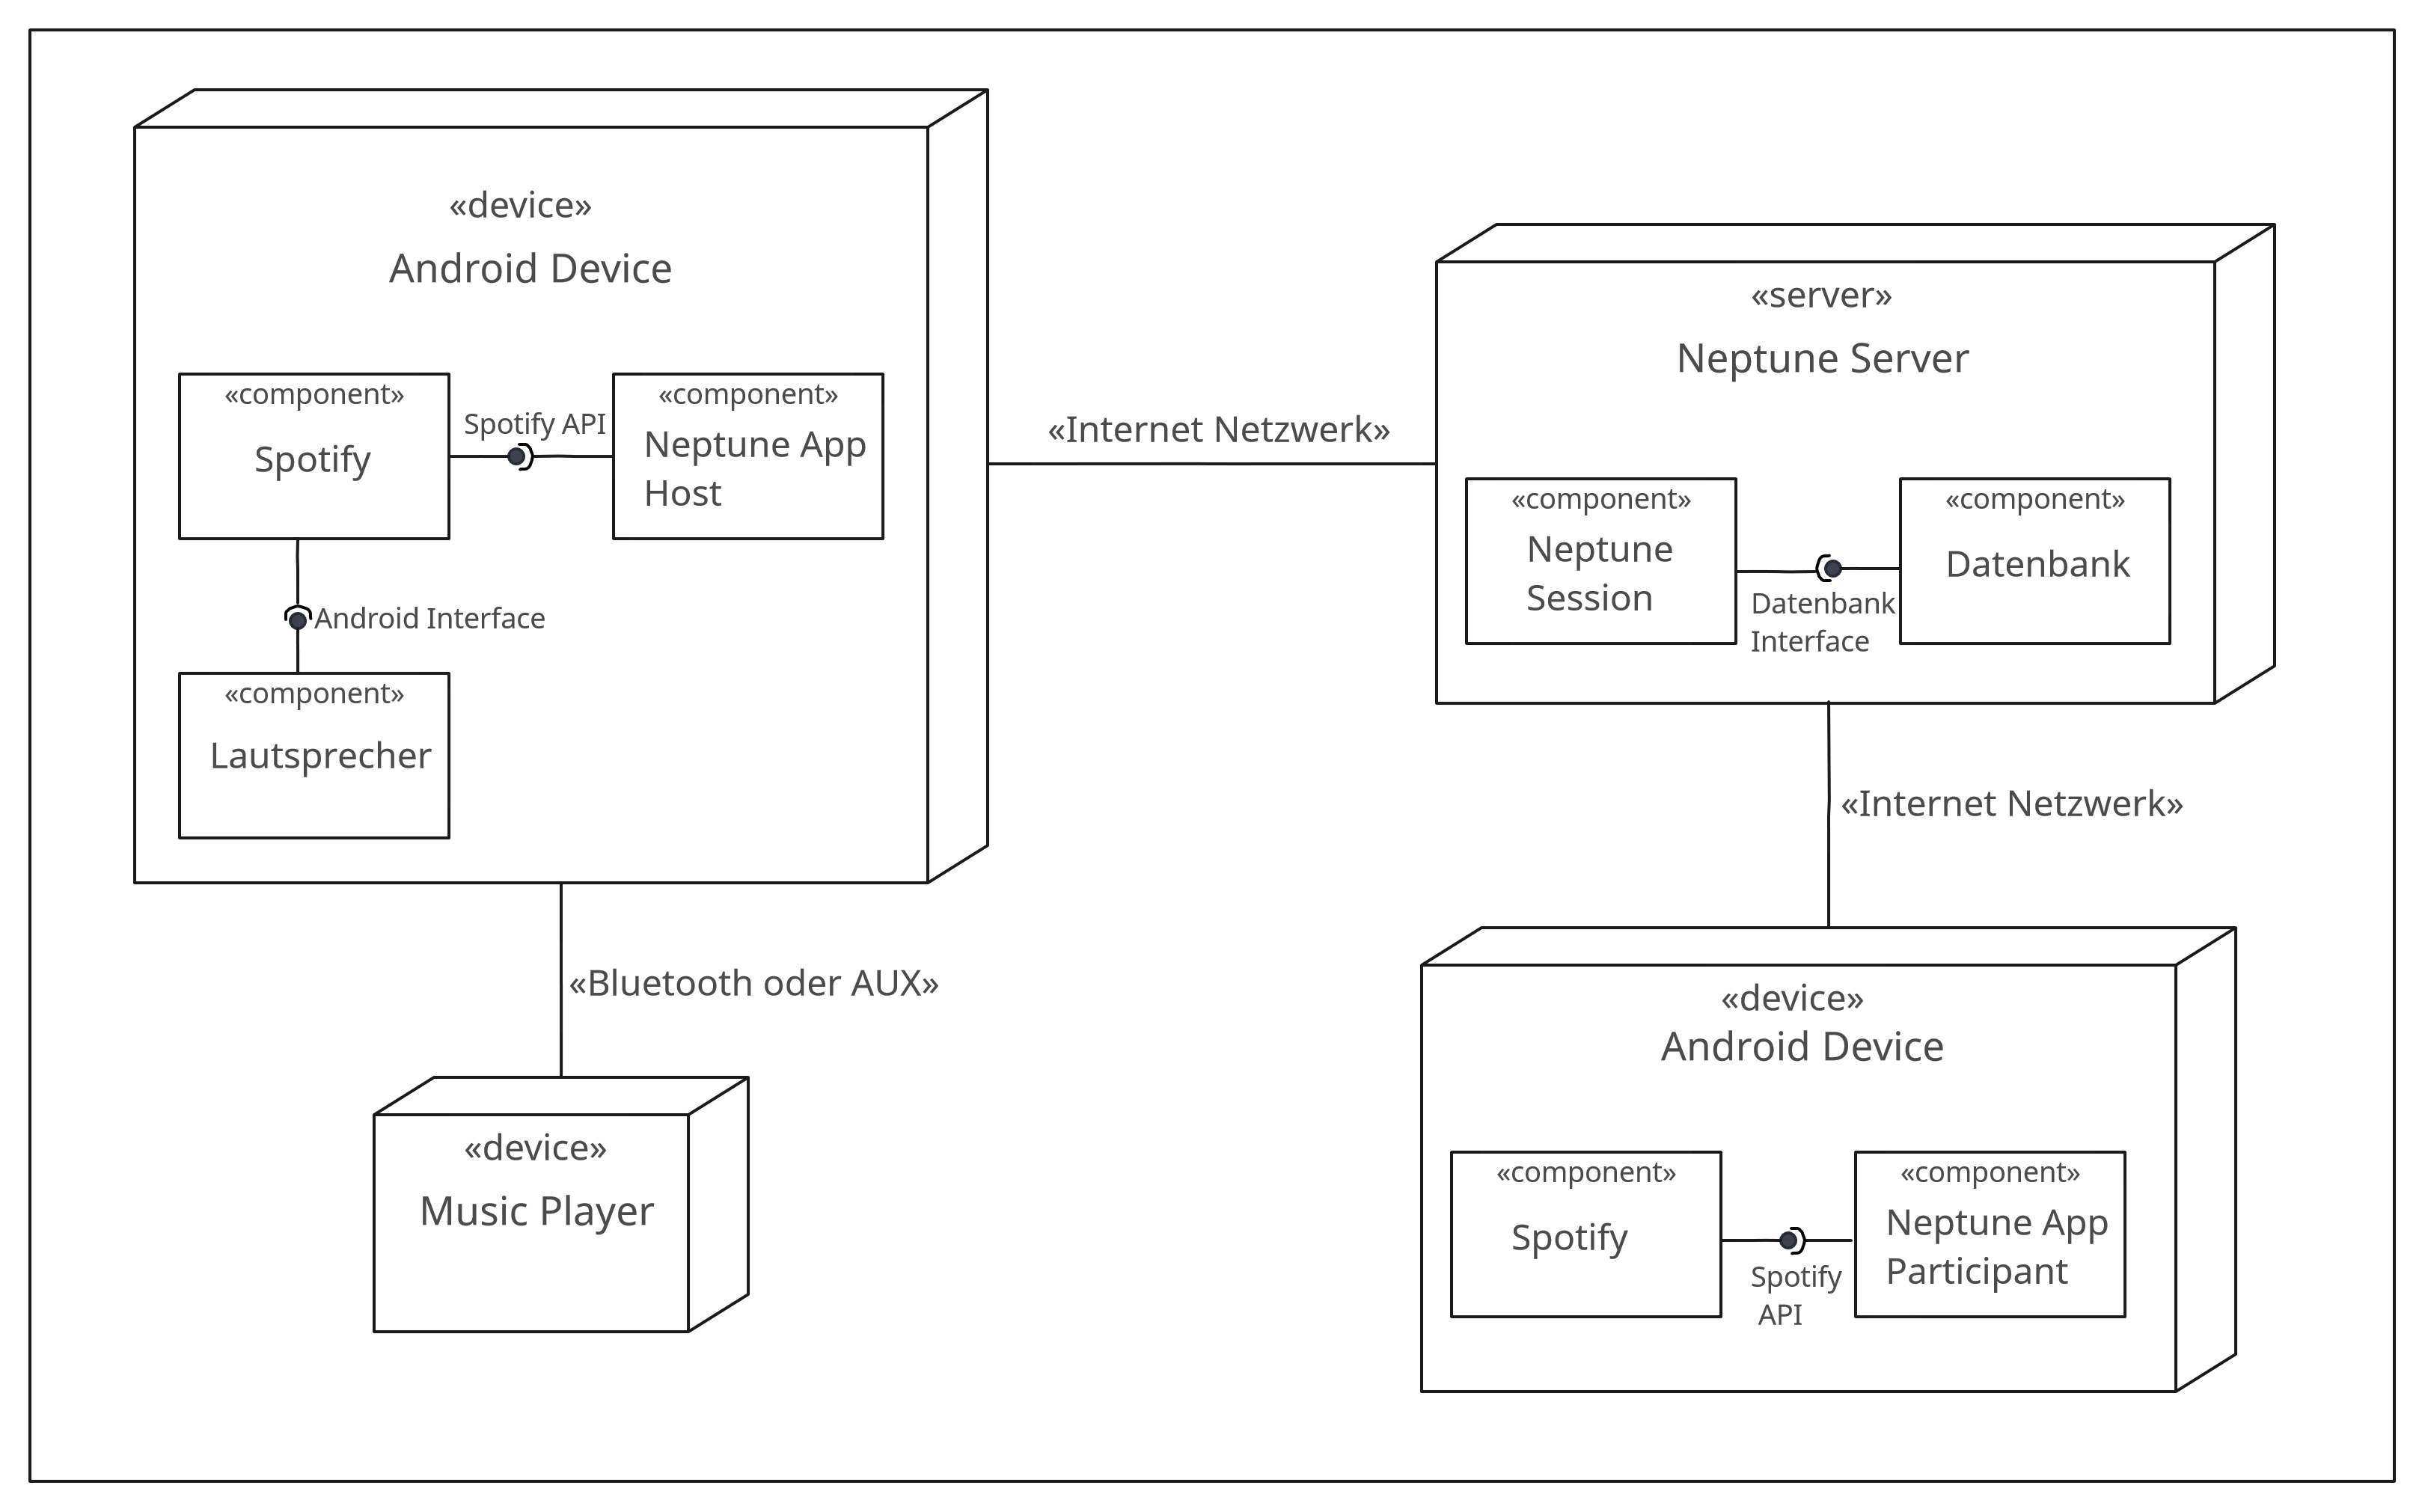
\includegraphics[width = 16cm]{LATEX/Pflichtenheft/GraphicDesigns/Verteilungsdiagramm.png}
    \caption{Verteilungsdiagramm}
    \label{fig:Verteilungsdiagramm}
\end{figure}



\chapter{Produktdaten}
\label{chap:Produktdaten}

\section{Systemdaten}
\label{sec:Produktdaten:Systemdaten}

Als Systemdaten werden sämtliche Daten zur Generierung der Benutzeroberfläche gespeichert, sowie die eindeutige Identifikation der App und Daten zum Auffinden des Servers. Zustandsdaten der App werden je nach Entwurfsentscheidung abgespeichert, um die App auch nach dem Schließen im selben Zustand erneut laden zu können. Es werden keinerlei Benutzereinstellungen oder Historiendaten gespeichert (SICHER ???). Auf dem Server werden Daten zum Zustand von Sessions gespeichert. Diese Session-Daten oder Teile von ihnen können auch kurzfristig lokal in der App der User gespeichert werden.

\section{Nutzerdaten}
\label{sec:Produktdaten:Nutzerdaten}

Es werden keinerlei sensiblen Nutzerdaten gespeichert. Im Fall des Musikdienstes Spotify müssen zur Verwendung der API keine Nutzerdaten gespeichert werden. Nur der generierte Nutzungstoken der API wird lokal gespeichert. Außerdem wird nach der Installation eine eindeutige Identifikation der App generiert, um User voneinander zu unterscheiden. Diese Identifikation wird lokal gespeichert und bei der Kommunikation von App und Server verwendet.



\chapter{Anforderungen an die App-Umgebung}
\label{chap:Appumgebung}

Wir stellen folgen Software und Hardware-Anforderungen an die App-Umgebung:

\begin{itemize}
    \item Als Gerät wird ein Smartphone oder gleichwertiges Gerät mit mindestens Android 7.0 benötigt.
    \item Eine jederzeit aktive Internetverbindung wird zur Nutzung der App-Funktionalität benötigt.
    \item Ein verknüpfter Spotify-Account wird benötigt, um als Full Participant an einer Session teilzunehmen.
    \item Ein verknüpfter Spotify-Premium-Account wird benötigt, um als Host eine Session zu erstellen und an ihr teilzunehmen.
\end{itemize}




\chapter{Tools und Ressourcen zur Entwicklung}
\label{chap:Entwicklungsumgebung}

\section{Software}
\label{sec:Entwicklungsumgebung:Software}

\begin{itemize}
    \item Entwicklung
    \begin{itemize}
        \item Android Studio Giraffe (2022.3.1)
    \end{itemize}
    
    \item Versionsverwaltung
    \begin{itemize}
        \item Git
        \item GitHub (zur Kommunikation)
    \end{itemize}

    \item UML Modellierung
    \begin{itemize}
        \item Creately
    \end{itemize}

    \item Grafikentwürfe
    \begin{itemize}
        \item PHPStorm
        \item GIMP
    \end{itemize}

    \item Sonstige Software
    \begin{itemize}
        \item Overleaf (für LATEX Dokumentation)
    \end{itemize}
    
\end{itemize}

\section{Hardware}
\label{sec:Entwicklungsumgebung:Hardware}

\begin{itemize}
    \item Diverse handelsübliche PCs und Laptops
    \item Diverse Android Smartphones mit mindestens Android 7.0
    \item Linux Rootserver
\end{itemize}



\chapter{Begriffserklärungen}
\label{chap:Begriffserklärungen}

\textbf{App}
 - Der Teil des Softwaresystems, der auf dem Android-Gerät des Nutzers läuft.

 \textbf{Full Participant}
 - Mit dem Musikdienst verknüpfter Participant, der Tracks im gesamten Katalog des Musikdienstes suchen kann.

\textbf{Host}
 - Ersteller einer Session, der (vorgeschlagene) Musik abspielt (kein Participant). Der Host benötigt ein Premium Abonnenment des Musikdienstes Spotify.

 \textbf{Musikdienst}
 - Der Musik-Streaminganbieter, über den die App Musik abspielt. Bei dieser App ist das Spotify.

 \textbf{Participant}
 - Teilnehmer einer Session (nicht der Host). Überbegriff für Full Participant und Restricted Participant.

 \textbf{Produkt}
 - Der Zustand, in dem das System nach Fertigstellung sein wird.

 \textbf{Queue}
 - Liste von Liedern, welche als nächstes durch den Musikdienst abgespielt werden.

 \textbf{Restricted Participant}
 - Nicht mit dem Musikdienst verknüpfter Participant, der nur Tracks von den bisher upgevoteten suchen kann.

 \textbf{Server}
 - Der Teil des Softwaresystems, der nicht auf dem Android-Gerät des Nutzers, sondern auf einem zentralen und externen Server läuft.

 \textbf{Session}
 - Eine Gruppe aus Participants und einem Host. In ihr können Tracks upgevotet und vom Host abgespielt werden.

\textbf{System}
 - Das gesamte zu entwickelnde Softwaresystem, Überbegriff von App und Server.

 \textbf{Track}
 - Lied bzw. Musikstück.

 \textbf{Upvote}
 - Bewertung auf einen Track. Je mehr Upvotes ein Track hat, desto beliebter ist er.

 \textbf{User}
 - Jeder Benutzer der App, Participant und Host sind User.

 \textbf{Vorschlagsliste}
 - Liste von Tracks einer Session, die mindestens ein Upvote haben.
 

\end{document}
